% !Mode:: "Tex:UTF-8"









\documentclass[10pt,a4paper]{article}
\usepackage{etoolbox}
\newtoggle{color}
%\togglefalse{color}
\toggletrue{color}

\usepackage{makeidx}
\newcommand{\idioma}{spanish}
\newcommand{\opcionesIdioma}{,es-nodecimaldot,es-tabla}
% !Mode:: "Tex:UTF-8"
%%%%%%%%%%%%%%%%%%%%%Carga de Packages
%%poner \newcommand{\idioma}{spanish} o \newcommand{\idioma}{english} en el documento
\usepackage{pdfsync}
\usepackage{srcltx}
\usepackage[\idioma\opcionesIdioma]{babel}
\usepackage[utf8x]{inputenc}
\usepackage[T1]{fontenc}
\usepackage{graphicx}
\graphicspath{{/users/fernando/figuras/}{./}{./figuras/}{/fernando/figuras/}{/fernando/figuras/jpg/}}
\usepackage{multicol}
\usepackage{epsfig}
%\usepackage{oberdiek}
\usepackage{listingsutf8}
\lstset{inputencoding=utf8/latin1}
%\lstset{extendedchars=true}
\lstset{ %
  language=R,                     % the language of the code
  basicstyle=\ttfamily\small,       % the size of the fonts that are used for the code
  numbers=left,                   % where to put the line-numbers
  numberstyle=\tiny\color{gray},  % the style that is used for the line-numbers
  stepnumber=1,                   % the step between two line-numbers. If it's 1, each line
                                  % will be numbered
  numbersep=5pt,                  % how far the line-numbers are from the code
  backgroundcolor=\color{white},  % choose the background color. You must add \usepackage{color}
  showspaces=false,               % show spaces adding particular underscores
  showstringspaces=false,         % underline spaces within strings
  showtabs=false,                 % show tabs within strings adding particular underscores
  frame=single,                   % adds a frame around the code
  rulecolor=\color{black},        % if not set, the frame-color may be changed on line-breaks within not-black text (e.g. commens (green here))
  tabsize=2,                      % sets default tabsize to 2 spaces
  %captionpos=,                   % sets the caption-position to bottom
  breaklines=true,                % sets automatic line breaking
  breakatwhitespace=false,        % sets if automatic breaks should only happen at whitespace
  %title=\lstname,                 % show the filename of files included with \lstinputlisting;
                                  % also try caption instead of title
  keywordstyle=\color{black},      % keyword style
  commentstyle=\color{Brown},   % comment style
  stringstyle=\color{black},      % string literal style
  escapeinside={\%*}{*)},         % if you want to add a comment within your code
  morekeywords={*,...},            % if you want to add more keywords to the set
  lineskip={-2.5pt} % single line spacing
}
%\usepackage{algorithm}
\usepackage{amsmath}
\usepackage{amsfonts}
\usepackage{amssymb}
\usepackage{amsthm}
\usepackage{fancybox}
\usepackage{fancyvrb}
\usepackage{rotating}
\usepackage{keystroke}
\usepackage{array}
\input{xy}
\xyoption{all}
%\usepackage[dvipsnames,usenames]{color}
\usepackage[usenames,dvipsnames,svgnames,table]{xcolor}
\usepackage{colortbl}
\usepackage{comment}
\excludecomment{spanish}
\excludecomment{english}
\includecomment{\idioma}

%\usepackage{noweb}
%\usepackage{clrscode}
\usepackage{eurosym}
\usepackage{wasysym}
\usepackage{multirow}
%\usepackage{margins}
\usepackage{lscape}
\usepackage{longtable}
\usepackage[normalem]{ulem}
\usepackage{xr-hyper}

%%NUEVO
\newcolumntype{C}{{\centering\arraybackslash}m{20mm}}
\newcommand{\centercell}[1]{\multicolumn{1}{c}{#1}}
\newcommand{\colHead}[1]{\centercell{\bfseries#1}}

\excludecomment{ocultar}


% Matriz (par‚ntesis)
\def\matr#1#2{\left(\begin{array}{#1}#2\end{array}\right)}
% Determinante (barras)
\def\deter#1#2{\left|\begin{array}{#1}#2\end{array}\right|}
% Sistema de ecuaciones. (llave a la izda.)
\def\seq#1#2{\left\{\begin{array}{#1}#2\end{array}\right.}
% Ecuaci\'on de varias lineas (sin llave a la izda.)
\def\evl#1#2{\begin{array}{#1}#2\end{array}}

%%%%%%%%%%%%%%%%%%%%%%%%%%%%%%%%%%%%%%%%%%%%%%
%%%%%%%%%%%%%%%%%%%%%%%%%%%%%%%%%%%%%%%%%%%%%%
%%%%%%%%%%%%%%%%% M\'{a}rgenes %%%%%%%%%%%%%%%%
%
%
%\parindent=0mm
%
%\textwidth=160mm
%\textheight=220mm
%\hoffset=-20mm
%\voffset=-15mm
%\parskip=0mm
\marginparsep=3mm
\marginparwidth=25mm
%
%%%%%%%%%%%%%%%%%%%%%%%%%%%% Contadores para listas de problemas
%\newcommand{\adc}{\addtocounter{enumi}{1}}
\newcommand{\adc}{\stepcounter{enumi}}
\newcommand{\adci}{\stepcounter{enumii}}
\newcommand{\xadc}{\addtocounter{xcounter}{1}}
\newcommand{\be}{\begin{enumerate}}
\newcommand{\ee}{\end{enumerate}}
\newcommand{\bi}{\begin{itemize}}
\newcommand{\ei}{\end{itemize}}
\newcounter{xcounter}


\newcommand{\nin}{{\noindent}}

%\newcounter{prob}{}
%\def\pr{\addtocounter{prob}{1}(\theprob)\ }
%\def\pr2{\addtocounter{prob}{2}(\theprob)\ }

%%%%%%%%%%%%%%%%%%%%%%%%%%%Fin de demostraciones, ejemplos, etc.
\newcommand{\fin}{$\square$}
%%%%%%%%%%%%%%%%%%%%%%%%%%Notaci\'{o}n matem\'{a}ticas generales
%\newcommand{\suc}[1]{\{#1_n\}}
%\newcommand{\sucn}[1]{\{#1_n\}_{n\in\mathbb{N}}}
%\newcommand{\ser}[1]{\sum #1_n}
%\newcommand{\sern}[1]{\sum_{n\geq 1} #1_n}
%\newcommand{\limn}{\lim_{n\rightarrow\infty}}
%\newcommand{\limnd}{\displaystyle\lim_{n\rightarrow\infty}}
%\newcommand{\mf}[1]{\mathbf{#1}}
%\newcommand{\mb}[1]{\mathbb{#1}}
%\newcommand{\D}[1]{\Dv_{\mf{#1}}}
%\newcommand{\bsigma}{\pmb{\sigma}}
%\newcommand{\bPhi}{\pmb{\Phi}}
%\newcommand{\vol}{\operatorname{vol}}
%\newcommand{\ldbr}{[\hspace{-1.5pt}[}
%\newcommand{\rdbr}{]\hspace{-1.5pt}]}
%\newcommand{\fpws}[2]{{#1}\ldbr{#2}\rdbr}
%\newcommand{\leftPui}{<\hspace{-3pt}<}
%\newcommand{\rightPui}{\hspace{-3pt}}
%\newcommand{\Pui}[2]{{#1}\hspace{-6pt}\leftPui{#2}\rightPui}
%\newcommand{\pdd}[2]{\dfrac{\partial{#1}}{\partial{#2}}}
%%%%%%%%%%Conjuntos de n\'{u}meros
\newcommand{\N}{\mathbb{N}} %conjunto de n\'{u}meros naturales
\newcommand{\Z}{\mathbb{Z}} %conjunto de n\'{u}meros enteros
\newcommand{\R}{\mathbb{R}} %conjunto de n\'{u}meros reales
\newcommand{\C}{\mathbb{C}} %conjunto de n\'{u}meros complejos
\newcommand{\Q}{\mathbb{Q}} %conjunto de n\'{u}meros racionales
\newcommand{\EP}{\mathbb{P}} %espacios proyectivos
\newcommand{\K}{\mathbb{K}} %cuerpo gen\'{e}rico
\newcommand{\A}{\mathbb{A}} %espacios afines

%%%%%%%%%%Estadistica
\newcommand{\MEAN}{\mathrm{E}}
\newcommand{\Var}{\mathrm{Var}}
\newcommand{\Cov}{\mathrm{Cov}}


%%%%%%%%%%Funciones
\def\arcsen{\operatorname{arcsen}}
\def\arctg{\operatorname{arctg}}
\def\argCosh{\operatorname{argCosh}}
\def\argSenh{\operatorname{argSenh}}
\def\argTgh{\operatorname{argTgh}}
\def\cosec{\operatorname{cosec}}
\def\Cosh{\operatorname{Cosh}}
\def\cotg{\operatorname{cotg}}
\def\Dv{\operatorname{D}}
\def\discrim{\operatorname{discrim}}
\def\dive{\operatorname{div}}
\def\dom{\operatorname{dom}}
\def\Ext{\operatorname{Ext}}
\def\Fr{\operatorname{Fr}}
\def\dder#1#2{\dfrac{d #1}{d #2} } %derivada en estilo display
\def\gr{\operatorname{gr}}
\def\grad{\operatorname{grad}}
\def\Imag{\operatorname{Im}}
\def\mcm{\operatorname{mcm}}
\def\rang{\operatorname{rang}}
\def\rot{\operatorname{rot}}
\def\sen{\operatorname{sen}}
\def\Senh{\operatorname{Senh}}
\def\sgn{\operatorname{sgn}}
\def\sig{\operatorname{sig}}
\def\tg{\operatorname{tg}}
\def\Tgh{\operatorname{Tgh}}
\def\E{\operatorname{E}}
\def\VAR{\operatorname{VAR}}
\newcommand{\margWeb}[2]{\noindent{#2}\marginpar[\hspace{-18mm}\link{#1}{WEB}]{\hspace*{-18mm}\link{#1}{WEB}}}

%%%%%%%%%%%%%%%%%%%%%%\'{A}lgebra conmutativa.
\def\multideg{\operatorname{multideg}} %multidegree of a polynomial
\def\LT{\operatorname{lt}} %leading term of a polynomial
\def\LC{\operatorname{lc}} %leading coefficient of a polynomial
\def\LM{\operatorname{lm}} %leading monomial of a polynomial
\def\Mexp{\mathbb{Z}^n_{\geq 0}} %set of multiexponents of monomials
\def\set#1{\left\{{#1}\right\}}
\newcommand{\vlist}[2]{\mbox{${#1}_{1},\ldots,{#1}_{#2}$}}
\def\deg{\operatorname{deg}} %grado de un polinomio
\def\cp{\operatorname{cp}} %coeficiente principal de un polinomio
\def\CP{\operatorname{cp}} %coeficiente principal de un polinomio
\def\set#1{\left\{{#1}\right\}} %llaves de conjunto
\newcommand{\V}{{\bf V}} %variedad de un conjunto de polinomios
\newcommand{\I}{{\bf I}} %ideal de un conjunto
\newcommand{\MCD}{\operatorname{mcd}} %m\'{a}ximo com\'{u}n divisor
\newcommand{\MCM}{\operatorname{mcm}} %m\'{\i}nimo com\'{u}n m\'{u}ltiplo
\newcommand{\LCM}{\operatorname{lcm}} %least common multiple
\newcommand{\GCD}{\operatorname{gcd}} %greatest common divisor
\newcommand{\Ker}{\operatorname{Ker}} %N\'{u}cleo
\newcommand{\IM}{\operatorname{IM}} %Imagen
\newcommand{\Rad}{\operatorname{Rad}} %radical de un ideal
\newcommand{\Jac}{\operatorname{Jac}} %radical de Jacobson de un anillo
\newcommand{\Ann}{\operatorname{Ann}} %anulador de un ideal
\newcommand{\Res}{\operatorname{Res}} %resultante de polinomios
\newcommand{\Mult}{\operatorname{mult}} %multiplicidad
\newcommand{\Gen}{\operatorname{Gen}} %g\'{e}nero
\newcommand{\Card}{\operatorname{Card}} %cardinal
\newcommand{\ord}{\operatorname{ord}} %orden
\newcommand{\prim}{\operatorname{prim}} %parte primitiva
\newcommand{\NP}{\operatorname{NP}} %NP idea
\newcommand{\cont}{\operatorname{cont}} %parte primitva
\newcommand{\pp}{\operatorname{pp}} %parte primitva
\newcommand{\PP}{\mathop{\mathrm{PP}}\nolimits}
\newcommand{\Int}{\operatorname{Int}}
\newcommand{\Ind}{\operatorname{index}}
\newcommand{\Lcoeff}{\operatorname{lc}} %leading coefficient of a polynomial
\newcommand{\Sqf}{\operatorname{Sqf}} %square free part of a polynomial

\def\pd#1#2{\frac{\partial #1}{\partial #2}} %derivada parcial
\def\mult{\text{mult}} %multiplicity
\def\Sing{\text{Sing}} %multiplicity
\def\Cl#1{\overline{#1}} %cierre topol\'{o}gico
\def\fobox#1{\begin{center}\fbox{$\displaystyle #1 $}\end{center}}

%\newcommand{\Ext}{\operatorname{Ext}}

%%%%%%%%%%%%%%%%%%%%%%%%
%% unpunto mayor que cdot, pero menor que bullet
\newcommand{\sbt}{\,\begin{picture}(-1,1)(-1,-3)\circle*{3}\end{picture}\ }

%%%%%%%%%%%%%%%%%%%%%%%%S\'{\i}mbolos rodeados de un c\'{\i}rculo
\def\circled#1{\xymatrix{*+[o][F]{#1}}}

%%%%%%%%%%%%%%%%%%%Geometr\'{\i}a
\newcommand{\CH}{{\cal CH}} %%cierre convexo

%%%%%%%%%%%%%%%%%%%%Tipos de letra especiales
%%Caligr\'{a}ficas
\newcommand{\cA}{{\cal A}}
\newcommand{\cB}{{\cal B}}
\newcommand{\cC}{{\cal C}}
\newcommand{\cD}{{\cal D}}
\newcommand{\cE}{{\cal E}}
\newcommand{\cF}{{\cal F}}
\newcommand{\cG}{{\cal G}}
\newcommand{\cH}{{\cal H}}
\newcommand{\cI}{{\cal I}}
\newcommand{\cJ}{{\cal J}}
\newcommand{\cK}{{\cal K}}
\newcommand{\cL}{{\cal L}}
\newcommand{\cM}{{\cal M}}
\newcommand{\cN}{{\cal N}}
\newcommand{\cO}{{\cal O}}
\newcommand{\cP}{{\cal P}}
\newcommand{\cQ}{{\cal Q}}
\newcommand{\cR}{{\cal R}}
\newcommand{\cS}{{\cal S}}
\newcommand{\cT}{{\cal T}}
\newcommand{\cU}{{\cal U}}
\newcommand{\cV}{{\cal V}}
\newcommand{\cW}{{\cal W}}
\newcommand{\cX}{{\cal X}}
\newcommand{\cY}{{\cal Y}}
\newcommand{\cZ}{{\cal Z}}

%%%%%%%%%%%%%%%%%%%%%%%%%%Notaci\'{o}n matem\'{a}ticas generales
\newcommand{\sucn}[1]{\{#1_n\}_{n\in\mathbb{N}}}
\newcommand{\ser}[1]{\sum #1_n}
\newcommand{\sern}[1]{\sum_{n\geq 1} #1_n}
\newcommand{\limn}{\lim_{n\rightarrow\infty}}
\newcommand{\mf}[1]{\mathbf{#1}}
\newcommand{\mb}[1]{\mathbb{#1}}
\newcommand{\D}[1]{\Dv_{\mf{#1}}}
\newcommand{\bsigma}{\pmb{\sigma}}
\newcommand{\bPhi}{\pmb{\Phi}}
\newcommand{\vol}{\operatorname{vol}}
\newcommand{\ldbr}{[\hspace{-1.5pt}[}
\newcommand{\rdbr}{]\hspace{-1.5pt}]}
\newcommand{\fpws}[2]{{#1}\ldbr{#2}\rdbr}
\newcommand{\leftPui}{<\hspace{-3pt}<}
\newcommand{\rightPui}{\hspace{-3pt}}
\newcommand{\Pui}[2]{{#1}\hspace{-6pt}\leftPui{#2}\rightPui}
\newcommand{\pdd}[2]{\dfrac{\partial{#1}}{\partial{#2}}}


%\newcounter{contEnlace}

%\newcommand{\pendiente}{\textcolor{purple}{PENDIENTE: }}
%\newcommand{\link}[2]{\textcolor{blue}{{\href{#1}{#2}}}}


\iftoggle{color}{%
  % color version
  \newcommand{\pendiente}{\textcolor{red}{PENDIENTE: }}
  \newcommand{\link}[2]{\textcolor{blue}{{\href{#1}{#2}}}}
  \newcommand{\fichero}[2]{\textattachfile{#1}{\textcolor{blue}{#2}}}
  \newcommand{\otrofichero}[2]{\textattachfile{./datos/#1}{\textcolor{blue}{#2}}}
}{%
  % b/w version
  \newcommand{\pendiente}{\textcolor{black}{\underline{PENDIENTE:} }}
  \newcommand{\link}[2]{\textcolor{black}{{\href{#1}{\underline{#2}}}}}
  \newcommand{\fichero}[2]{\textattachfile{#1}{\textcolor{black}{\underline{#2}}}}
  \newcommand{\otrofichero}[2]{\textattachfile{./datos/#1}{\textcolor{black}{\underline{#2}}}}
}



%{\textcolor{blue}{{\href{#1}{#2}}}}

%%%%%%%%%%%%%%%%%%COLORES

\DefineNamedColor{named}{Brown}{cmyk}{0,0.81,1,0.60}
\definecolor{Gris050}{gray}{0.50}
\definecolor{Gris025}{gray}{0.75}
\definecolor{Gris010}{gray}{0.90}


%%%%%%%%%%%%%%%%%%%%%Package Algorithms
%\begin{spanish}
%\renewcommand{\algorithmicrequire}{{precondici\'{o}n:}}
%\renewcommand{\algorithmicensure}{{postcondici\'{o}n:}}
%\renewcommand{\algorithmicend}{{fin}}
%\renewcommand{\algorithmicif}{{si}}
% \renewcommand{\algorithmicthen}{{entonces}}
% \renewcommand{\algorithmicelse}{{si no}}
% \renewcommand{\algorithmicelsif}{\algorithmicelse\ \algorithmicif}
% \renewcommand{\algorithmicendif}{\algorithmicend\ \algorithmicif}
% \renewcommand{\algorithmicfor}{{para}}
% \renewcommand{\algorithmicforall}{{para todo}}
% \renewcommand{\algorithmicdo}{{hacer}}
% \renewcommand{\algorithmicendfor}{\algorithmicend\ \algorithmicfor}
% \renewcommand{\algorithmicwhile}{{mientras}}
% \renewcommand{\algorithmicendwhile}{\algorithmicend\ \algorithmicwhile}
% \renewcommand{\algorithmicrepeat}{{repetir}}
% \renewcommand{\algorithmicuntil}{{hasta}}
% \end{spanish}

%%%%%%%%%%%%%%%%%%%%%%%%%%%%%%%%%%Package Amsthm
\begin{spanish}
%\theoremstyle{definition}% default
\theoremstyle{plain}
\newtheorem{thm}{Teorema}[section]
\newtheorem{teo}{Teorema}[section]
\newtheorem{teorema}{Teorema}[section]
\newtheorem{lem}[thm]{Lema}
\newtheorem{lema}[thm]{Lema}
\newtheorem{prop}[thm]{Proposici\'{o}n}
\newtheorem{proposicion}[thm]{Proposici\'{o}n}
\newtheorem{cor}[thm]{Corolario}
\newtheorem{corolario}[thm]{Corolario}
\newtheorem*{KL}{Klein's Lemma}
%\theoremstyle{definition}
\newtheorem{defn}[thm]{Definici\'{o}n}
\newtheorem{definicion}[thm]{Definici\'{o}n}
\newtheorem{conj}[thm]{Conjetura}
\newtheorem{conjetura}[thm]{Conjetura}
\newtheorem{definicionInformal}[thm]{Definición Informal}
\newtheorem{exmp}[thm]{Ejemplo}
\newtheorem{ejemplo}[thm]{Ejemplo}
\newtheorem{Ejemplo}[thm]{Ejemplo}
\newtheorem{ejem}[thm]{Ejemplo}
\newtheorem{ejercicio}{Ejercicio}
%\theoremstyle{remark}
\newtheorem*{rem}{Observaci\'{o}n}
\newtheorem{observacion}[thm]{Observaci\'{o}n}
\newtheorem*{note}{Nota}
\newtheorem{nota}[thm]{Nota}
\newtheorem{case}[thm]{Caso}
\newtheorem{caso}[thm]{Caso}
\newtheorem{regla}[thm]{Regla}

\theoremstyle{remark}
\newtheorem{enlace}{$\bullet$ }
\end{spanish}

\begin{english}
\theoremstyle{plain}% default
%\theoremstyle{definition}
\newtheorem{thm}{Theorem}[section]
\newtheorem{lem}[thm]{Lemma}
\newtheorem{prop}[thm]{Proposition}
\newtheorem{cor}[thm]{Corollary}
\newtheorem*{KL}{Klein's Lemma}
\newtheorem{defn}[thm]{Definition}
\newtheorem{conj}[thm]{Conjecture}
\newtheorem{exmp}[thm]{Example}
\theoremstyle{remark}
\newtheorem*{rem}{Remark}
\newtheorem*{note}{Note}
\newtheorem{case}{Case}
\end{english}

%%%%%%%%%%%%%%%Package Listings
%\lstset{showstringspaces=false}
%\newcommand{\PAS}[1]{\lstinline@#1@}
%\newcommand{\CPP}[1]{\lstinline@#1@}


%%%%%%%%%%%%Estilo para bibliograf\'{\i}a

%\bibliographystyle{plain}

%%%%%%%%%%%%Mis anotaciones
\newcommand{\Pendiente}[1]{\textcolor{red}{Pendiente: #1}}
%\newcommand{\Pendiente}{\textcolor{purple}{Pendiente: }}

\newcommand{\fernando}[1]{\textcolor{red}{Fernando: #1}}

%%%%%%%%%%%%%%%% Enlace al indice
%\renewcommand{\chaptermark}[1]{\markboth{\chaptername\ \thechapter.#1 \ref{index}}{}}

%%%%%%%%%%%%%%%%%%Traducci\'{o}n de clrscode
%\renewcommand{\For}{\textbf{Para} }
%\renewcommand{\To}{\textbf{hasta} }
%\renewcommand{\By}{\textbf{incremento} }
%\renewcommand{\Downto}{\textbf{downto} }
%\renewcommand{\While}{\textbf{mientras} }
%\renewcommand{\Repeat}{\textbf{repetir}\\\addtocounter{indent}{1}}
%\renewcommand{\Until}{\kill\addtocounter{indent}{-1}\liprint\\\textbf{hasta que}\hspace*{-0.7em}\'}
%\renewcommand{\If}{\textbf{si} }
%\renewcommand{\Then}{\\textbf{entonces}\hspace{13mm}\\addtocounter{indent}{1}}
%\renewcommand{\Else}{\kill\addtocounter{indent}{-1}\liprint\\textbf{sino}\\addtocounter{indent}{1}}
%\renewcommand{\End}{\addtocounter{indent}{-1}}
%\renewcommand{\ElseIf}{\kill\addtocounter{indent}{-1}\liprint\textbf{sino si} }
%\renewcommand{\ElseNoIf}{\kill\addtocounter{indent}{-1}\liprint\textbf{si no}\addtocounter{indent}{1}}
%\renewcommand{\Do}{\\\textbf{hacer}\hspace*{-0.7em}\'\addtocounter{indent}{1}}
%\renewcommand{\Return}{\textbf{devolver} }
%\renewcommand{\Comment}{$\hspace*{-0.075em}\rhd$ }
%\renewcommand{\RComment}{\`\Comment}
%\renewcommand{\Goto}{\textbf{Ir a} }
%\renewcommand{\Error}{\textbf{error} }


%%%%%%%%%%%%%%%%%%%%%%%%%%%%%%%%%%%%%%%%%%%%%%%%%%%%%%%%%%%%%%%
%Cabecera para ejercicios
%\documentclass[11pt]{article}
%\newcommand{\idioma}{spanish}
%\input definiciones
%
%\textwidth=160mm \textheight=240mm \hoffset=-20mm \voffset=-30mm
%%\parskip=0mm
%%\marginparsep=-25mm \evensidemargin=82pt\evensidemargin=44pt
%
%
%\includecomment{solucion}
%%\excludecomment{solucion}

%%Compatibilidad con documentos antiguos
\newcounter{prob}{}
\def\pr{\noindent\addtocounter{prob}{1}(\theprob)\ }
\def\bepro{ \setcounter{prob}{0}}

%%Compatibilidad con documentos antiguos
% \def\ojo#1{
% \noindent$\btr$#1
% \marginpar[
% {GeoGebra}]
% {GeoGebra}}

% \def\atencion#1{\noindent #1
% \marginpar[
% {\includegraphics*[scale=1,width=1.2cm,keepaspectratio=true]{./datos/hipoizda}}]
% {\includegraphics*[scale=1,width=1.2cm,keepaspectratio=true]{./datos/hipodcha}}}


\def\Rlogo#1{\noindent #1
\marginpar[
{\includegraphics*[scale=1,width=1.5cm,keepaspectratio=true]{./datos/Rlogo.jpg}}]
{\includegraphics*[scale=1,width=1.5cm,keepaspectratio=true]{./datos/Rlogo.jpg}}}

\def\calcLogo#1{#1}

%\def\calcLogo#1{\noindent #1
%\marginpar[
%{\includegraphics*[scale=1,width=1.2cm,keepaspectratio=true]{./datos/LogoHojaCalculo.png}}]
%{\includegraphics*[scale=1,width=1.2cm,keepaspectratio=true]{./datos/LogoHojaCalculo.png}}}


\def\ninja#1{\noindent #1
\marginpar[ {\includegraphics*[scale=1,width=1.2cm,keepaspectratio=true]{../fig/ninja_desk.png}}]
{\includegraphics*[scale=1,width=1.2cm,keepaspectratio=true]{../fig/ninja_desk.png}}}

\def\buda#1{\noindent #1
\marginpar[ {\includegraphics*[scale=1,width=1.2cm,keepaspectratio=true]{../fig/Computer-Buddha.png}}]
{\includegraphics*[scale=1,width=1.2cm,keepaspectratio=true]{../fig/Computer-Buddha.png}}}


\def\puffin#1{\noindent #1
\marginpar[ {\includegraphics*[scale=1,width=1.2cm,keepaspectratio=true]{../fig/frailecillo3.png}}]
{\includegraphics*[scale=1,width=1.2cm,keepaspectratio=true]{../fig/frailecillo3-dcha.png}}}


\def\atencion{
\marginpar[
{\includegraphics*[scale=1,width=2cm,keepaspectratio=true]{./datos/hipoizda}}]
{\includegraphics*[scale=1,width=2cm,keepaspectratio=true]{./datos/hipodcha}}}


\def\ojo#1{
\noindent #1
\marginpar[
{\includegraphics*[scale=1,width=1.5cm,keepaspectratio=true]{./datos/hipoojoi}}]
{\includegraphics*[scale=1,width=1.5cm,keepaspectratio=true]{./datos/hipoojod}}}

\def\ojo2{
\marginpar[
{\includegraphics*[scale=1,width=1.5cm,keepaspectratio=true]{./datos/hipoojoi}}]
{\includegraphics*[scale=1,width=1.5cm,keepaspectratio=true]{./datos/hipoojod}}}


\def\lio#1{
\noindent$\btr$#1
\marginpar{\includegraphics*[scale=1,width=1.1cm,keepaspectratio=true]{./datos/hipolio}}}

\def\cuentas{
\marginpar{\includegraphics*[scale=1,width=1.3cm,keepaspectratio=true]{./datos/hipocuen}}}

\def\pensar{
\marginpar{\includegraphics*[scale=1,width=1.5cm,keepaspectratio=true]{./datos/hipopens}}}

\def\facil{
\marginpar{\includegraphics*[scale=1,width=2cm,keepaspectratio=true]{./datos/hipofcil}}}



\newcommand{\WikipediaLogo}{\marginpar{\includegraphics*[scale=1,width=1.2cm,keepaspectratio=true]{./datos/LogoWikipedia}}}
\newcommand{\MoodleLogo}{\marginpar{\includegraphics*[scale=1,width=1.2cm,keepaspectratio=true]{./datos/MoodleLogo}}}
\newcommand{\WirisGeoGebraLogo}{\marginpar{\includegraphics*[scale=1,width=1.2cm,keepaspectratio=true]{./datos/WirisGeoGebraLogo}}}
\newcommand{\WirisLogo}{\marginpar{\includegraphics*[scale=1,width=1.2cm,keepaspectratio=true]{./datos/WirisLogo}}}
\newcommand{\GeoGebraLogo}{\marginpar{\includegraphics*[scale=1,width=1.2cm,keepaspectratio=true]{./datos/GeoGebra-Logo}}}


\newcommand{\enObras}[1]{\includegraphics*[scale=1,width=0.5cm,keepaspectratio=true]{./datos/obras.png}\textcolor{blue}{#1}}



\newcommand{\GeoGebra}[2]{\noindent #1
\marginpar[{\link{#2}{\small Moodle}\\\includegraphics*[scale=1,width=1.2cm,keepaspectratio=true]{./datos/MoodleLogo}}]{\link{#2}{\small Moodle}\\\includegraphics*[scale=1,width=1.2cm,keepaspectratio=true]{./datos/MoodleLogo}}}

\newcommand{\Moodle}[2]{\noindent #1
\marginpar[{\link{#2}{\small Moodle}\\\includegraphics*[scale=1,width=1.2cm,keepaspectratio=true]{./datos/MoodleLogo}}]{\link{#2}{\small Moodle}\\\includegraphics*[scale=1,width=1.2cm,keepaspectratio=true]{./datos/MoodleLogo}}}

\newcommand{\Wikipedia}[2]{\noindent #1
\marginpar[{\link{#2}{\small Wikipedia}\\\includegraphics*[scale=1,width=1.2cm,keepaspectratio=true]{./datos/LogoWikipedia}}]{\link{#2}{\small Wikipedia}\\\includegraphics*[scale=1,width=1.2cm,keepaspectratio=true]{./datos/LogoWikipedia}}}


\newcommand{\pder}[2]{\frac{\partial #1}{\partial #2}}

%%%%%%%%%%%%%%%%%%%%%%%%%%%%%%%%%%%%%%%%%%%%%%
%%%%%%%%%%%%%%%%%%%%%%%%%%%%%%%%%%%%%%%%%%%%%%%
%%%%%%%%%%%%%%%%%% M\'{a}rgenes %%%%%%%%%%%%%%%%
%%
%%
%%\parindent=0mm
%%
%\textwidth=160mm \textheight=220mm \hoffset=-20mm \voffset=-15mm
%\parskip=0mm
%\marginparsep=-25mm
%%
%%%%%%%%%%%%%%%%%%%%%%%%%%%%% Contadores para listas de problemas
%%\newcommand{\adc}{\addtocounter{enumi}{1}}
%\newcommand{\adc}{\stepcounter{enumi}}
%\newcommand{\adci}{\stepcounter{enumii}}
%\newcommand{\xadc}{\addtocounter{xcounter}{1}}
%\newcommand{\be}{\begin{enumerate}}
%\newcommand{\ee}{\end{enumerate}}
%\newcommand{\bi}{\begin{itemize}}
%\newcommand{\ei}{\end{itemize}}
%\newcounter{xcounter}
%\newcounter{probl}
%\setcounter{probl}{0}
%\newcommand{\pro}{\addtocounter{probl}{1}}
%\newcommand{\pr}{{\pro}{(\theprobl.)}}
%%%%%%%%%%%%%%%%%%%%%%%%%%%%Fin de demostraciones, ejemplos, etc.
%\newcommand{\fin}{$\square$}
%%%%%%%%%%%%%%%%%%%%%%%%%%%Notaci\'{o}n matem\'{a}ticas generales
%\newcommand{\suc}[1]{\{#1_n\}}
%\newcommand{\sucn}[1]{\{#1_n\}_{n\in\mathbb{N}}}
%\newcommand{\ser}[1]{\sum #1_n}
%\newcommand{\sern}[1]{\sum_{n\geq 1} #1_n}
%\newcommand{\limn}{\lim_{n\rightarrow\infty}}
%\newcommand{\mf}[1]{\mathbf{#1}}
%\newcommand{\mb}[1]{\mathbb{#1}}
%\newcommand{\D}[1]{\Dv_{\mf{#1}}}
%\newcommand{\bsigma}{\pmb{\sigma}}
%\newcommand{\bPhi}{\pmb{\Phi}}
%\newcommand{\vol}{\operatorname{vol}}
%\newcommand{\ldbr}{[\hspace{-1.5pt}[}
%\newcommand{\rdbr}{]\hspace{-1.5pt}]}
%\newcommand{\fpws}[2]{{#1}\ldbr{#2}\rdbr}
%\newcommand{\leftPui}{<\hspace{-3pt}<}
%\newcommand{\rightPui}{\hspace{-3pt}}
%\newcommand{\Pui}[2]{{#1}\hspace{-6pt}\leftPui{#2}\rightPui}
%\newcommand{\pdd}[2]{\dfrac{\partial{#1}}{\partial{#2}}}
%%%%%%%%%%%Conjuntos de n\'{u}meros
%\newcommand{\N}{\mathbb{N}} %conjunto de n\'{u}meros naturales
%\newcommand{\Z}{\mathbb{Z}} %conjunto de n\'{u}meros enteros
%\newcommand{\R}{\mathbb{R}} %conjunto de n\'{u}meros reales
%\newcommand{\C}{\mathbb{C}} %conjunto de n\'{u}meros complejos
%\newcommand{\Q}{\mathbb{Q}} %conjunto de n\'{u}meros racionales
%\newcommand{\EP}{\mathbb{P}} %espacios proyectivos
%\newcommand{\K}{\mathbb{K}} %cuerpo gen\'{e}rico
%\newcommand{\A}{\mathbb{A}} %espacios afines
%%%%%%%%%%%Funciones
%\def\arcsen{\operatorname{arcsen}}
%\def\arctg{\operatorname{arctg}}
%\def\argCosh{\operatorname{argCosh}}
%\def\argSenh{\operatorname{argSenh}}
%\def\argTgh{\operatorname{argTgh}}
%\def\cosec{\operatorname{cosec}}
%\def\Cosh{\operatorname{Cosh}}
%\def\cotg{\operatorname{cotg}}
%\def\Dv{\operatorname{D}}
%\def\discrim{\operatorname{discrim}}
%\def\dive{\operatorname{div}}
%\def\dom{\operatorname{dom}}
%\def\Ext{\operatorname{Ext}}
%\def\Fr{\operatorname{Fr}}
%\def\gr{\operatorname{gr}}
%\def\grad{\operatorname{grad}}
%\def\Imag{\operatorname{Im}}
%\def\mcm{\operatorname{mcm}}
%\def\rang{\operatorname{rang}}
%\def\rot{\operatorname{rot}}
%\def\sen{\operatorname{sen}}
%\def\Senh{\operatorname{Senh}}
%\def\sgn{\operatorname{sgn}}
%\def\sig{\operatorname{sig}}
%\def\tg{\operatorname{tg}}
%\def\Tgh{\operatorname{Tgh}}
%\def\E{\operatorname{E}}
%\def\VAR{\operatorname{VAR}}
%
%%%%%%%%%%%%%%%%%%%%%%%\'{A}lgebra conmutativa.
%\def\multideg{\operatorname{multideg}} %multidegree of a polynomial
%\def\LT{\operatorname{lt}} %leading term of a polynomial
%\def\LC{\operatorname{lc}} %leading coefficient of a polynomial
%\def\LM{\operatorname{lm}} %leading monomial of a polynomial
%\def\Mexp{\mathbb{Z}^n_{\geq 0}} %set of multiexponents of monomials
%\def\set#1{\left\{{#1}\right\}}
%\newcommand{\vlist}[2]{\mbox{${#1}_{1},\ldots,{#1}_{#2}$}}
%\def\deg{\operatorname{deg}} %grado de un polinomio
%\def\cp{\operatorname{cp}} %coeficiente principal de un polinomio
%\def\CP{\operatorname{cp}} %coeficiente principal de un polinomio
%\def\set#1{\left\{{#1}\right\}} %llaves de conjunto
%\newcommand{\V}{{\bf V}} %variedad de un conjunto de polinomios
%\newcommand{\I}{{\bf I}} %ideal de un conjunto
%\newcommand{\MCD}{\operatorname{mcd}} %m\'{a}ximo com\'{u}n divisor
%\newcommand{\MCM}{\operatorname{mcm}} %m\'{\i}nimo com\'{u}n m\'{u}ltiplo
%\newcommand{\LCM}{\operatorname{lcm}} %least common multiple
%\newcommand{\GCD}{\operatorname{gcd}} %greatest common divisor
%\newcommand{\Ker}{\operatorname{Ker}} %N\'{u}cleo
%\newcommand{\IM}{\operatorname{IM}} %Imagen
%\newcommand{\Rad}{\operatorname{Rad}} %radical de un ideal
%\newcommand{\Jac}{\operatorname{Jac}} %radical de Jacobson de un anillo
%\newcommand{\Ann}{\operatorname{Ann}} %anulador de un ideal
%\newcommand{\Res}{\operatorname{Res}} %resultante de polinomios
%\newcommand{\Mult}{\operatorname{mult}} %multiplicidad
%\newcommand{\Gen}{\operatorname{Gen}} %g\'{e}nero
%\newcommand{\Card}{\operatorname{Card}} %cardinal
%\newcommand{\ord}{\operatorname{ord}} %orden
%\newcommand{\prim}{\operatorname{prim}} %parte primitiva
%\newcommand{\NP}{\operatorname{NP}} %NP idea
%\newcommand{\cont}{\operatorname{cont}} %parte primitva
%\newcommand{\pp}{\operatorname{pp}} %parte primitva
%\newcommand{\PP}{\mathop{\mathrm{PP}}\nolimits}
%\newcommand{\Int}{\operatorname{Int}}
%\newcommand{\Ind}{\operatorname{index}}
%\newcommand{\Lcoeff}{\operatorname{lc}} %leading coefficient of a polynomial
%\newcommand{\Sqf}{\operatorname{Sqf}} %square free part of a polynomial
%
%\def\pd#1#2{\frac{\partial #1}{\partial #2}} %derivada parcial
%\def\mult{\text{mult}} %multiplicity
%\def\Sing{\text{Sing}} %multiplicity
%\def\Cl#1{\overline{#1}} %cierre topol\'{o}gico
%
%%\newcommand{\Ext}{\operatorname{Ext}}
%
%%%%%%%%%%%%%%%%%%%%%%%%%S\'{\i}mbolos rodeados de un c\'{\i}rculo
%\def\circled#1{\xymatrix{*+[o][F]{#1}}}
%
%%%%%%%%%%%%%%%%%%%%Geometr\'{\i}a
%\newcommand{\CH}{{\cal CH}} %%cierre convexo
%
%%%%%%%%%%%%%%%%%%%%%Tipos de letra especiales
%%%Caligr\'{a}ficas
%\newcommand{\cA}{{\cal A}}
%\newcommand{\cB}{{\cal B}}
%\newcommand{\cC}{{\cal C}}
%\newcommand{\cD}{{\cal D}}
%\newcommand{\cE}{{\cal E}}
%\newcommand{\cF}{{\cal F}}
%\newcommand{\cG}{{\cal G}}
%\newcommand{\cH}{{\cal H}}
%\newcommand{\cI}{{\cal I}}
%\newcommand{\cJ}{{\cal J}}
%\newcommand{\cK}{{\cal K}}
%\newcommand{\cL}{{\cal L}}
%\newcommand{\cM}{{\cal M}}
%\newcommand{\cN}{{\cal N}}
%\newcommand{\cO}{{\cal O}}
%\newcommand{\cP}{{\cal P}}
%\newcommand{\cQ}{{\cal Q}}
%\newcommand{\cR}{{\cal R}}
%\newcommand{\cS}{{\cal S}}
%\newcommand{\cT}{{\cal T}}
%\newcommand{\cU}{{\cal U}}
%\newcommand{\cV}{{\cal V}}
%\newcommand{\cW}{{\cal W}}
%\newcommand{\cX}{{\cal X}}
%\newcommand{\cY}{{\cal Y}}
%\newcommand{\cZ}{{\cal Z}}
%
%
%%%%%%%%%%%%%%%%%%%COLORES
%
%\DefineNamedColor{named}{Brown}{cmyk}{0,0.81,1,0.60}
%\definecolor{Gris050}{gray}{0.50}
%\definecolor{Gris025}{gray}{0.50}
%
%
%%\theoremstyle{plain}
%%\newtheorem{thm}{Teorema}[section]
%%%\newtheorem{teo}{Teorema}[section]
%%\newtheorem{lem}[thm]{Lema}
%%\newtheorem{prop}[thm]{Proposici\'{o}n}
%%\newtheorem{cor}[thm]{Corolario}
%%\newtheorem*{KL}{Klein's Lemma}
%%%\theoremstyle{definition}
%%\newtheorem{defn}[thm]{Definici\'{o}n}
%%\newtheorem{conj}[thm]{Conjetura}
%%\newtheorem{exmp}[thm]{Ejemplo}
%%\newtheorem{ejem}[thm]{Ejemplo}
%%\theoremstyle{remark}
%%\newtheorem*{rem}{Observaci\'{o}n}
%%\newtheorem*{note}{Nota}
%%\newtheorem{case}{Caso}
%%\newtheorem{regla}[thm]{Regla}
%
%\theoremstyle{plain}
%\newtheorem{thm}{Teorema}%[subsection]
%%\newtheorem{teo}{Teorema}[section]
%%\newtheorem{teorema}{Teorema}[section]
%\newtheorem{lem}[thm]{Lema}
%\newtheorem{lema}[thm]{Lema}
%\newtheorem{prop}[thm]{Proposici\'{o}n}
%\newtheorem{proposicion}[thm]{Proposici\'{o}n}
%\newtheorem{cor}[thm]{Corolario}
%\newtheorem{corolario}[thm]{Corolario}
%\newtheorem*{KL}{Klein's Lemma}
%%\theoremstyle{definition}
%\newtheorem{defn}[thm]{Definici\'{o}n}
%\newtheorem{definicion}[thm]{Definici\'{o}n}
%\newtheorem{conj}[thm]{Conjetura}
%\newtheorem{conjetura}[thm]{Conjetura}
%\newtheorem{exmp}[thm]{Ejemplo}
%\newtheorem{ejemplo}[thm]{Ejemplo}
%\newtheorem{ejem}[thm]{Ejemplo}
%\newtheorem{ejercicio}[thm]{Ejemplo}
%\theoremstyle{remark}
%\newtheorem*{rem}{Observaci\'{o}n}
%\newtheorem*{observacion}{Observaci\'{o}n}
%\newtheorem*{note}{Nota}
%\newtheorem*{nota}{Nota}
%\newtheorem{case}{Caso}
%\newtheorem{caso}{Caso}
%\newtheorem{regla}[thm]{Regla}
%
%%%%%%%%%%%%%Estilo para bibliograf\'{\i}a
%
%\bibliographystyle{plain}
%
%%%%%%%%%%%%%Mis anotaciones
%\newcommand{\Pendiente}{\textcolor{blue}{Pendiente: }}

\renewcommand{\listtablename}{Indice de tablas}
\renewcommand{\tablename}{Tabla}


%%%%%%%%%%%%%%%%%%%%%%%%%%%%%%%%%%%%%%%%%%%%%%%%%%%
\def\indexCond#1{
\ifnumcomp{\value{chapter}}{<}{3}{
        \index{#1}
    }
    {
        \index{#1}%% nothing is done
    }
}


\usepackage[pageanchor=true]{hyperref}
\makeindex

\usepackage{pdfpages}

%\input{sahp}
\includecomment{com}
%\excludecomment{com}
%\usepackage[dvips]{hyperref}
%\usepackage{pstricks}


\newtoggle{distribuir}
%\togglefalse{distribuir}
\toggletrue{distribuir}
\iftoggle{distribuir}{%
  % color version
    \includecomment{distribuir}
    \excludecomment{noDistribuir}
}{%
  % b/w version
    \includecomment{noDistribuir}
    \excludecomment{distribuir}
}


\usepackage{attachfile}

\textwidth=150mm \textheight=260mm
\hoffset=-1cm
\voffset=-25mm
\parskip=2mm
%\textwidth=160mm \textheight=240mm \hoffset=-20mm \voffset=-20mm \parskip=0mm \marginparsep=-25mm

\setlength{\parindent}{0pt}
\newcounter {cont01}

\externaldocument[curso-]{../CursoIntroduccionEstadistica/000-CursoEstadistica}
\externaldocument[tut01-]{Tutorial-01}
\externaldocument[tut02-]{Tutorial-02}
\externaldocument[tut03-]{Tutorial-03}
\externaldocument[tut04-]{Tutorial-04}
\externaldocument[tut05-]{Tutorial-05}
\externaldocument[tut06-]{Tutorial-06}
\externaldocument[tut07-]{Tutorial-07}
\externaldocument[tut08-]{Tutorial-08}
\externaldocument[tut08-]{Tutorial-09}
\externaldocument[tut08-]{Tutorial-10}
\externaldocument[tut08-]{Tutorial-11}
\externaldocument[tut08-]{Tutorial-12}

\begin{document}
\includecomment{pdf}
%\excludecomment{pdf}
%\includecomment{dvi}
\excludecomment{dvi}
%\includecomment{com}
\excludecomment{com}

\paragraph{\link{http://www.postdata-statistics.com/}{PostData}\hspace{6.3cm}Curso de Introducci<U+00F3>n a la Estad<U+00ED>stica\\[2mm]} \noindent\hrule

\setcounter{section}{0}
\section*{\hspace{-0.1cm}\fbox{\colorbox{Gris025}{
\begin{minipage}{14.5cm}
Tutorial 13: Regresi<U+00F3>n log<U+00ED>stica.
\end{minipage}
}}} Atenci<U+00F3>n:
\begin{itemize}
  \item Este documento pdf lleva adjuntos algunos de los ficheros de datos necesarios. Y est<U+00E1>
      pensado para trabajar con <U+00E9>l directamente en tu ordenador. Al usarlo en la pantalla, si es
      necesario, puedes aumentar alguna de las figuras para ver los detalles. Antes de
      imprimirlo, piensa si es necesario. Los <U+00E1>rboles y nosotros te lo agradeceremos.
  \item Fecha: \today. Si este fichero tiene m<U+00E1>s de un a<U+00F1>o, puede resultar obsoleto. Busca si
      existe una versi<U+00F3>n m<U+00E1>s reciente.
\end{itemize}
\setcounter{tocdepth}{1}
\tableofcontents

\section{Construcci<U+00F3>n de un modelo de regresi<U+00F3>n log<U+00ED>stica con R.}

En esta secci<U+00F3>n vamos a  ver c<U+00F3>mo utilizar R para obtener un modelo de regresi<U+00F3>n log<U+00ED>stica, partiendo de datos como los del Ejemplo \ref{curso-cap13:ejem:RegresionLogistica00} (p<U+00E1>g. \pageref{curso-cap13:ejem:RegresionLogistica00}) del libro. As<U+00ED> que empezaremos por leer esos datos a partir del fichero que los contiene:
% Como en tutoriales anteriores, vamos a trabajar con un fichero plantilla que contiene  el c<U+00F3>digo necesario para reproducir los resultados m<U+00E1>s importantes del an<U+00E1>lisis que vamos a realizar a continuaci<U+00F3>n. El fichero es:
% \begin{center}
% \fichero{../datos/Tut13-RegresionLogistica.R}{Tut13-RegresionLogistica.R}
% \end{center}
% Te recomendamos
%cuyo listado puedes ver en la Tabla \ref{Tut13:tabla:FicheroR-RegresionLogistica.R} de la p<U+00E1>g. \pageref{Tut13:tabla:FicheroR-RegresionLogistica.R}.







\begin{knitrout}
\definecolor{shadecolor}{rgb}{0.969, 0.969, 0.969}\color{fgcolor}\begin{kframe}
\begin{alltt}
\hlstd{datosFichero} \hlkwb{=} \hlkwd{read.table}\hlstd{(}\hlstr{"../datos/Cap13-DatosVasculopatia.csv"}\hlstd{,}
                          \hlkwc{header} \hlstd{=} \hlnum{TRUE}\hlstd{,} \hlkwc{sep}\hlstd{=}\hlstr{","}\hlstd{)}
\hlkwd{head}\hlstd{(datosFichero)}
\end{alltt}
\begin{verbatim}
##    ITB Vasculopatia
## 1 0.94            0
## 2 0.99            0
## 3 0.88            1
## 4 0.64            1
## 5 1.25            0
## 6 0.50            1
\end{verbatim}
\end{kframe}
\end{knitrout}

El resultado de la lectura es un {\tt data.frame} de R en el que tenemos dos variables (columnas), llamadas {\tt ITB} y {\tt Vasculopatia}, respectivamente. En lo que sigue vamos a utilizar el nombre $X$ para la variable explicativa e $Y$ para la variable respuesta, que es un factor. Suponemos que $X$ aparece en la primera columna del {\tt data.frame} mientras que {\tt Y} ocupa la segunda columna. Como en el caso del Anova, puede suceder que el orden de columnas en el fichero {\tt csv} no coincida con este. Pero en cualquier caso, podemos ajustar ese comportamiento cambiando a $2$ el valor de la variable {\tt colX}.

\begin{knitrout}
\definecolor{shadecolor}{rgb}{0.969, 0.969, 0.969}\color{fgcolor}\begin{kframe}
\begin{alltt}
\hlstd{colX} \hlkwb{=} \hlnum{1}
\hlkwa{if}\hlstd{(colX} \hlopt{==} \hlnum{1}\hlstd{)\{}
  \hlstd{X} \hlkwb{=} \hlstd{datosFichero[ ,} \hlnum{1}\hlstd{]}
  \hlstd{Y} \hlkwb{=} \hlstd{datosFichero[ ,} \hlnum{2}\hlstd{]}
\hlstd{\}} \hlkwa{else} \hlstd{\{}
  \hlstd{X} \hlkwb{=} \hlstd{datosFichero[ ,} \hlnum{2}\hlstd{]}
  \hlstd{Y} \hlkwb{=} \hlstd{datosFichero[ ,} \hlnum{1}\hlstd{]}
\hlstd{\}}
\hlstd{datos} \hlkwb{=} \hlkwd{data.frame}\hlstd{(X, Y)}
\end{alltt}
\end{kframe}
\end{knitrout}

Ya tenemos los datos listos para el an<U+00E1>lisis. El diagrama de dispersi<U+00F3>n correspondiente se obtiene con:




{\small
\begin{knitrout}
\definecolor{shadecolor}{rgb}{0.969, 0.969, 0.969}\color{fgcolor}\begin{kframe}
\begin{alltt}
\hlstd{colores} \hlkwb{=} \hlkwd{c}\hlstd{()}
\hlstd{colores[datos}\hlopt{$}\hlstd{Y} \hlopt{==} \hlnum{0}\hlstd{]} \hlkwb{=} \hlstr{"grey"}
\hlstd{colores[datos}\hlopt{$}\hlstd{Y} \hlopt{==} \hlnum{1}\hlstd{]} \hlkwb{=} \hlstr{"black"}
\hlkwd{plot}\hlstd{(datos}\hlopt{$}\hlstd{X, datos}\hlopt{$}\hlstd{Y,} \hlkwc{pch} \hlstd{=} \hlnum{21}\hlstd{,} \hlkwc{bg} \hlstd{= colores,} \hlkwc{cex}\hlstd{=}\hlnum{1.3}\hlstd{,}\hlkwc{font}\hlstd{=}\hlnum{2}\hlstd{,}
     \hlkwc{xlab} \hlstd{=} \hlstr{"Indice tobillo brazo"}\hlstd{,} \hlkwc{ylab} \hlstd{=} \hlstr{"Vasculopatia"}\hlstd{,} \hlkwc{font.lab}\hlstd{=}\hlnum{2}\hlstd{, )}
\hlkwd{legend}\hlstd{(}\hlstr{"left"}\hlstd{,} \hlkwd{c}\hlstd{(}\hlstr{"No vasculopat<U+00ED>a"}\hlstd{,} \hlstr{"Vasculopat<U+00ED>a"}\hlstd{),} \hlkwc{pch} \hlstd{=} \hlnum{21}\hlstd{,}
       \hlkwc{pt.bg} \hlstd{=}  \hlkwd{c}\hlstd{(}\hlstr{"grey"}\hlstd{,} \hlstr{"black"}\hlstd{))}
\hlkwd{box}\hlstd{(}\hlkwc{lwd}\hlstd{=}\hlnum{3}\hlstd{)}
\end{alltt}
\end{kframe}

{\centering \includegraphics[width=\maxwidth]{figure/diagramaDispersionEjemplo-1} 

}



\end{knitrout}
}

En la Secci<U+00F3>n \ref{curso-cap13:sec:IntroduccionProblemaRegresionLogistica} del libro (p<U+00E1>g. \pageref{curso-cap13:sec:IntroduccionProblemaRegresionLogistica})
hemos visto tambi<U+00E9>n un modelo ficticio en el que existe un umbral claramente definido de valores de $X$ (por ejemplo, $X=0.96$) a partir del cual todos los valores de $Y$ son $0$, mientras que antes son $1$. Por si te interesa, esa situaci<U+00F3>n se puede reproducir f<U+00E1>cilmente en el c<U+00F3>digo as<U+00ED>:

\begin{knitrout}
\definecolor{shadecolor}{rgb}{0.969, 0.969, 0.969}\color{fgcolor}\begin{kframe}
\begin{alltt}
\hlstd{Ysimul01} \hlkwb{=} \hlkwd{ifelse}\hlstd{(X} \hlopt{>} \hlnum{0.96}\hlstd{,} \hlkwc{yes} \hlstd{=} \hlnum{0}\hlstd{,} \hlkwc{no} \hlstd{=} \hlnum{1}\hlstd{)}
\hlstd{datosSimul01} \hlkwb{=} \hlkwd{data.frame}\hlstd{(X,} \hlkwc{Y} \hlstd{= Ysimul01)}
\end{alltt}
\end{kframe}
\end{knitrout}
Y entonces su diagrama es:
\begin{knitrout}
\definecolor{shadecolor}{rgb}{0.969, 0.969, 0.969}\color{fgcolor}\begin{kframe}
\begin{alltt}
\hlstd{colores} \hlkwb{=} \hlkwd{c}\hlstd{()}
\hlstd{colores[datosSimul01}\hlopt{$}\hlstd{Y} \hlopt{==} \hlnum{0}\hlstd{]} \hlkwb{=} \hlstr{"grey"}
\hlstd{colores[datosSimul01}\hlopt{$}\hlstd{Y} \hlopt{==} \hlnum{1}\hlstd{]} \hlkwb{=} \hlstr{"black"}
\hlkwd{plot}\hlstd{(datosSimul01}\hlopt{$}\hlstd{X, datosSimul01}\hlopt{$}\hlstd{Y,} \hlkwc{pch} \hlstd{=} \hlnum{21}\hlstd{,} \hlkwc{bg} \hlstd{= colores,} \hlkwc{cex}\hlstd{=}\hlnum{1.3}\hlstd{,}\hlkwc{font}\hlstd{=}\hlnum{2}\hlstd{,}
     \hlkwc{xlab} \hlstd{=} \hlstr{"Indice tobillo brazo"}\hlstd{,} \hlkwc{ylab} \hlstd{=} \hlstr{"Vasculopatia"}\hlstd{,} \hlkwc{font.lab}\hlstd{=}\hlnum{2}\hlstd{, )}
\hlkwd{legend}\hlstd{(}\hlstr{"left"}\hlstd{,} \hlkwd{c}\hlstd{(}\hlstr{"No vasculopat<U+00ED>a"}\hlstd{,} \hlstr{"Vasculopat<U+00ED>a"}\hlstd{),} \hlkwc{pch} \hlstd{=} \hlnum{21}\hlstd{,} \hlkwc{pt.bg} \hlstd{=}  \hlkwd{c}\hlstd{(}\hlstr{"grey"}\hlstd{,} \hlstr{"black"}\hlstd{))}
\hlkwd{box}\hlstd{(}\hlkwc{lwd}\hlstd{=}\hlnum{3}\hlstd{)}
\end{alltt}
\end{kframe}

{\centering \includegraphics[width=\maxwidth]{figure/diagramaSimul01-1} 

}



\end{knitrout}
La figura sim<U+00E9>trica, cuando $Y=1$ corresponde a valores altos de $X$ se obtiene de forma similar.

Por <U+00FA>ltimo, la figura correspondiente al caso ``todo ruido, nada de modelo'' se obtiene simplemente eligiendo al azar los valores de $Y$:

\begin{knitrout}
\definecolor{shadecolor}{rgb}{0.969, 0.969, 0.969}\color{fgcolor}\begin{kframe}
\begin{alltt}
\hlkwd{set.seed}\hlstd{(}\hlnum{2015}\hlstd{)}
\hlstd{Ysimul03} \hlkwb{=} \hlkwd{sample}\hlstd{(}\hlnum{0}\hlopt{:}\hlnum{1}\hlstd{,} \hlkwc{size} \hlstd{=} \hlkwd{length}\hlstd{(X),} \hlkwc{replace} \hlstd{=} \hlnum{TRUE}\hlstd{)}
\hlstd{datosSimul03} \hlkwb{=} \hlkwd{data.frame}\hlstd{(X,} \hlkwc{Y} \hlstd{= Ysimul03)}
\hlstd{colores} \hlkwb{=} \hlkwd{c}\hlstd{()}
\hlstd{colores[datosSimul03}\hlopt{$}\hlstd{Y} \hlopt{==} \hlnum{0}\hlstd{]} \hlkwb{=} \hlstr{"grey"}
\hlstd{colores[datosSimul03}\hlopt{$}\hlstd{Y} \hlopt{==} \hlnum{1}\hlstd{]} \hlkwb{=} \hlstr{"black"}
\hlkwd{plot}\hlstd{(datosSimul03}\hlopt{$}\hlstd{X, datosSimul03}\hlopt{$}\hlstd{Y,} \hlkwc{pch} \hlstd{=} \hlnum{21}\hlstd{,} \hlkwc{bg} \hlstd{= colores,} \hlkwc{cex}\hlstd{=}\hlnum{1.3}\hlstd{,}\hlkwc{font}\hlstd{=}\hlnum{2}\hlstd{,}
     \hlkwc{xlab} \hlstd{=} \hlstr{"Indice tobillo brazo"}\hlstd{,} \hlkwc{ylab} \hlstd{=} \hlstr{"Vasculopatia"}\hlstd{,} \hlkwc{font.lab}\hlstd{=}\hlnum{2}\hlstd{, )}
\hlkwd{legend}\hlstd{(}\hlstr{"left"}\hlstd{,} \hlkwd{c}\hlstd{(}\hlstr{"No vasculopat<U+00ED>a"}\hlstd{,} \hlstr{"Vasculopat<U+00ED>a"}\hlstd{),} \hlkwc{pch} \hlstd{=} \hlnum{21}\hlstd{,} \hlkwc{pt.bg} \hlstd{=}  \hlkwd{c}\hlstd{(}\hlstr{"grey"}\hlstd{,} \hlstr{"black"}\hlstd{))}
\hlkwd{box}\hlstd{(}\hlkwc{lwd}\hlstd{=}\hlnum{3}\hlstd{)}
\end{alltt}
\end{kframe}

{\centering \includegraphics[width=\maxwidth]{figure/diagramaSimul03-1} 

}



\end{knitrout}

\subsection{Agrupando valores para estimar las probabilidades.}
\label{tut13:subsec:ConstruccionDetalladaModelo}

 Vamos ahora a ver ahora detalladamente como usar R para dar los pasos 1 a 4 del Ejemplo \ref{curso-cap13:ejem:EstimacionModeloLogisticoMedianteClases} del libro (p<U+00E1>g. \pageref{curso-cap13:ejem:EstimacionModeloLogisticoMedianteClases}). El primer paso es la lectura de los datos desde el fichero, que incluimos aqu<U+00ED> por comodidad:
\begin{center}
\fichero{../datos/Cap13-ConstruccionModeloLogistico.csv}{Cap13-ConstruccionModeloLogistico.csv}
\end{center}
Una vez descargado este fichero en nuestra carpeta {\tt datos},  usamos read.table para leerlo y luego procedemos como con el anterior ejemplo (ten en cuenta que los datos de este fichero est<U+00E1>n separados con tabuladores, por eso usamos \verb# sep = \t#)

\begin{knitrout}
\definecolor{shadecolor}{rgb}{0.969, 0.969, 0.969}\color{fgcolor}\begin{kframe}
\begin{alltt}
\hlstd{datosFichero} \hlkwb{=} \hlkwd{read.table}\hlstd{(}\hlstr{"../datos/Cap13-ConstruccionModeloLogistico.csv"}\hlstd{,}
                          \hlkwc{header} \hlstd{=} \hlnum{TRUE}\hlstd{,} \hlkwc{sep}\hlstd{=}\hlstr{"\textbackslash{}t"}\hlstd{)}
\hlkwd{head}\hlstd{(datosFichero)}
\end{alltt}
\begin{verbatim}
##       X Y
## 1 -3.83 0
## 2 -2.85 0
## 3 -6.23 0
## 4  8.57 1
## 5 -8.14 0
## 6 -4.93 0
\end{verbatim}
\end{kframe}
\end{knitrout}
Como antes, fijamos los nombres de las variables y pintamos el diagrama de dispersi<U+00F3>n:
\begin{knitrout}
\definecolor{shadecolor}{rgb}{0.969, 0.969, 0.969}\color{fgcolor}

{\centering \includegraphics[width=\maxwidth]{figure/unnamed-chunk-3-1} 

}



\end{knitrout}

Los valores de la variable $X$ est<U+00E1>n comprendidos completamente en el intervalo $[-10, 10]$:
\begin{knitrout}
\definecolor{shadecolor}{rgb}{0.969, 0.969, 0.969}\color{fgcolor}\begin{kframe}
\begin{alltt}
\hlkwd{range}\hlstd{(X)}
\end{alltt}
\begin{verbatim}
## [1] -9.98 10.00
\end{verbatim}
\end{kframe}
\end{knitrout}

Vamos con los pasos del 1 al 4 del ejemplo:
\begin{enumerate}

\item Empezamos dividiendo el intervalo $[-10, 10]$ en $40$ clases de anchura $\frac{1}{2}$ y localizando los puntos de corte que marcan las fronteras entre clases, que son los valores $u_0, \ldots, u_{40}$ del ejemplo. Hay que prestar atenci<U+00F3>n al n<U+00FA>mero de valores que generamos: $41$ puntos definen $40$ clases.

\begin{knitrout}
\definecolor{shadecolor}{rgb}{0.969, 0.969, 0.969}\color{fgcolor}\begin{kframe}
\begin{alltt}
\hlstd{a} \hlkwb{=} \hlopt{-}\hlnum{10}
\hlstd{b} \hlkwb{=}  \hlnum{10}
\hlstd{numClases} \hlkwb{=} \hlnum{40}
\hlstd{(u} \hlkwb{=} \hlkwd{seq}\hlstd{(}\hlkwc{from}\hlstd{=a,} \hlkwc{to}\hlstd{=b,} \hlkwc{length.out}\hlstd{=(numClases} \hlopt{+} \hlnum{1}\hlstd{)))} \hlcom{# Fronteras entre clases}
\end{alltt}
\begin{verbatim}
##  [1] -10.0  -9.5  -9.0  -8.5  -8.0  -7.5  -7.0  -6.5  -6.0  -5.5  -5.0
## [12]  -4.5  -4.0  -3.5  -3.0  -2.5  -2.0  -1.5  -1.0  -0.5   0.0   0.5
## [23]   1.0   1.5   2.0   2.5   3.0   3.5   4.0   4.5   5.0   5.5   6.0
## [34]   6.5   7.0   7.5   8.0   8.5   9.0   9.5  10.0
\end{verbatim}
\end{kframe}
\end{knitrout}

Las marcas de clase, que en el libro hemos llamado $w_i$, son los puntos medios de cada intervalo. Se obtienen f<U+00E1>cilmente sumando a cada valor {\tt u} la semianchura de la clase. Hay que tener cuidado de nuevo con el n<U+00FA>mero de marcas de clase que generamos:
\begin{knitrout}
\definecolor{shadecolor}{rgb}{0.969, 0.969, 0.969}\color{fgcolor}\begin{kframe}
\begin{alltt}
\hlstd{(marcasClase} \hlkwb{=}  \hlstd{(u} \hlopt{+} \hlstd{((b} \hlopt{-} \hlstd{a)} \hlopt{/} \hlstd{(}\hlnum{2} \hlopt{*} \hlstd{numClases)))[}\hlnum{1}\hlopt{:}\hlstd{numClases])}
\end{alltt}
\begin{verbatim}
##  [1] -9.75 -9.25 -8.75 -8.25 -7.75 -7.25 -6.75 -6.25 -5.75 -5.25 -4.75
## [12] -4.25 -3.75 -3.25 -2.75 -2.25 -1.75 -1.25 -0.75 -0.25  0.25  0.75
## [23]  1.25  1.75  2.25  2.75  3.25  3.75  4.25  4.75  5.25  5.75  6.25
## [34]  6.75  7.25  7.75  8.25  8.75  9.25  9.75
\end{verbatim}
\end{kframe}
\end{knitrout}

\item Ahora vamos a hacer un recuento de cu<U+00E1>ntos de los valores $X$ caen en cada una de esas clases. Afortunadamente, ya sabemos que en R esto es muy f<U+00E1>cil de hacer, usando la funci<U+00F3>n {\tt cut} para definir un factor que clasifique los valores de $X$:

\begin{knitrout}
\definecolor{shadecolor}{rgb}{0.969, 0.969, 0.969}\color{fgcolor}\begin{kframe}
\begin{alltt}
\hlstd{clases} \hlkwb{=} \hlkwd{cut}\hlstd{(X,} \hlkwc{breaks}\hlstd{=u,} \hlkwc{include.lowest}\hlstd{=}\hlnum{TRUE}\hlstd{)}
\end{alltt}
\end{kframe}
\end{knitrout}
La opci<U+00F3>n {\tt include.lowest=TRUE} sirve para que el primer intervalo sea cerrado a la izquierda, cubriendo as<U+00ED> los posibles valores de $X=-10$ (aunque nuestra muestra, en este ejemplo, no incluye ninguno de esos valores). Veamos los primeros valores del factor; puedes compararlos con los primeros valores de $X$ para ver qu<U+00E9> la clasificaci<U+00F3>n es correcta:
\begin{knitrout}
\definecolor{shadecolor}{rgb}{0.969, 0.969, 0.969}\color{fgcolor}\begin{kframe}
\begin{alltt}
\hlkwd{head}\hlstd{(clases,} \hlnum{10}\hlstd{)}
\end{alltt}
\begin{verbatim}
##  [1] (-4,-3.5] (-3,-2.5] (-6.5,-6] (8.5,9]   (-8.5,-8] (-5,-4.5] (5,5.5]  
##  [8] (9.5,10]  (9.5,10]  (5,5.5]  
## 40 Levels: [-10,-9.5] (-9.5,-9] (-9,-8.5] (-8.5,-8] ... (9.5,10]
\end{verbatim}
\begin{alltt}
\hlkwd{head}\hlstd{(X,} \hlnum{10}\hlstd{)}
\end{alltt}
\begin{verbatim}
##  [1] -3.83 -2.85 -6.23  8.57 -8.14 -4.93  5.03  9.92  9.78  5.48
\end{verbatim}
\end{kframe}
\end{knitrout}
El recuento que nos hab<U+00ED>amos propuesto consiste simplemente en hacer una tabla de frecuencias del factor {\tt clases}
\begin{knitrout}
\definecolor{shadecolor}{rgb}{0.969, 0.969, 0.969}\color{fgcolor}\begin{kframe}
\begin{alltt}
\hlkwd{table}\hlstd{(clases)}
\end{alltt}
\begin{verbatim}
## clases
## [-10,-9.5]  (-9.5,-9]  (-9,-8.5]  (-8.5,-8]  (-8,-7.5]  (-7.5,-7] 
##         25         33         21         13         27         29 
##  (-7,-6.5]  (-6.5,-6]  (-6,-5.5]  (-5.5,-5]  (-5,-4.5]  (-4.5,-4] 
##         29         20         30         19         23         31 
##  (-4,-3.5]  (-3.5,-3]  (-3,-2.5]  (-2.5,-2]  (-2,-1.5]  (-1.5,-1] 
##         22         26         26         21         27         17 
##  (-1,-0.5]   (-0.5,0]    (0,0.5]    (0.5,1]    (1,1.5]    (1.5,2] 
##         25         26         21         31         25         21 
##    (2,2.5]    (2.5,3]    (3,3.5]    (3.5,4]    (4,4.5]    (4.5,5] 
##         28         34         28         31         16         31 
##    (5,5.5]    (5.5,6]    (6,6.5]    (6.5,7]    (7,7.5]    (7.5,8] 
##         28         27         26         27         23         22 
##    (8,8.5]    (8.5,9]    (9,9.5]   (9.5,10] 
##         25         23         22         21
\end{verbatim}
\end{kframe}
\end{knitrout}
Como se dice en el libro, puedes constatar en esta tabla que hay $27$ puntos de la muestra con
\[-8<X\leq -7.5.\]

La Tabla \ref{curso-cap13:tabla:Clase18EjemploModeloMedianteClases} del libro (p<U+00E1>g. \pageref{curso-cap13:tabla:Clase18EjemploModeloMedianteClases}) contiene, a modo de ejemplo, los valores de $X$ que caen en la clase n<U+00FA>mero 18 y los correspondientes valores de $Y$. Para obtener esos valores en R podemos hacer:
\begin{knitrout}
\definecolor{shadecolor}{rgb}{0.969, 0.969, 0.969}\color{fgcolor}\begin{kframe}
\begin{alltt}
\hlstd{(claseElegida} \hlkwb{=} \hlkwd{levels}\hlstd{(clases)[}\hlnum{18}\hlstd{])}
\end{alltt}
\begin{verbatim}
## [1] "(-1.5,-1]"
\end{verbatim}
\begin{alltt}
\hlstd{X[clases} \hlopt{==} \hlstd{claseElegida]}
\end{alltt}
\begin{verbatim}
##  [1] -1.02 -1.13 -1.35 -1.15 -1.23 -1.43 -1.00 -1.34 -1.01 -1.04 -1.06
## [12] -1.42 -1.06 -1.07 -1.05 -1.25 -1.12
\end{verbatim}
\begin{alltt}
\hlstd{(cualesSon} \hlkwb{=} \hlkwd{which}\hlstd{(clases} \hlopt{==} \hlstd{claseElegida))}
\end{alltt}
\begin{verbatim}
##  [1]  29  53  75  97 122 139 303 465 573 607 655 659 737 743 833 880 968
\end{verbatim}
\begin{alltt}
\hlstd{X[cualesSon]}
\end{alltt}
\begin{verbatim}
##  [1] -1.02 -1.13 -1.35 -1.15 -1.23 -1.43 -1.00 -1.34 -1.01 -1.04 -1.06
## [12] -1.42 -1.06 -1.07 -1.05 -1.25 -1.12
\end{verbatim}
\begin{alltt}
\hlstd{Y[cualesSon]}
\end{alltt}
\begin{verbatim}
##  [1] 0 0 1 0 1 1 0 0 0 1 0 0 0 0 1 1 0
\end{verbatim}
\end{kframe}
\end{knitrout}

\begin{ejercicio}
\label{tut13:ejercicio01}
Comprueba que, como se dice en el libro, la clase n<U+00FA>mero $5$ es el intervalo $(-8,-7.5]$. Comprueba tambi<U+00E9>n que esa clase contiene $27$ puntos y que los valores $Y$ de esos $27$ puntos muestrales son {\em todos} iguales a $0$. Haz un estudio similar con la clase n<U+00FA>mero $35$.
%Soluciones en la p<U+00E1>gina \pageref{tut13:ejercicio01:sol}.
\qed
\end{ejercicio}


\item A continuaci<U+00F3>n, para estimar las probabilidades correspondientes a cada una de esas clases vamos a utilizar la funci<U+00F3>n {\tt tapply}. Esta funci<U+00F3>n nos permite aplicar una funci<U+00F3>n (en este caso  la suma) a todos los elementos de un vector (o matriz, o array) agrupados mediante un cierto factor. En nuestro ejemplo eso se traduce en una frase como:

{\em
``Calcular la suma (aplicar la funci<U+00F3>n {\tt sum}) de todos los valores del vector {\tt Y}, agrup<U+00E1>ndolos primero por clases (con la opci<U+00F3>n {\tt INDEX=clases})''.
}

Guardaremos los resultados en un vector de R llamado {\tt sumaYporClases}:
\begin{knitrout}
\definecolor{shadecolor}{rgb}{0.969, 0.969, 0.969}\color{fgcolor}\begin{kframe}
\begin{alltt}
\hlstd{(sumaYporClases} \hlkwb{=} \hlkwd{tapply}\hlstd{(Y,} \hlkwc{INDEX}\hlstd{=clases,} \hlkwc{FUN}\hlstd{=sum))}
\end{alltt}
\begin{verbatim}
## [-10,-9.5]  (-9.5,-9]  (-9,-8.5]  (-8.5,-8]  (-8,-7.5]  (-7.5,-7] 
##          0          0          0          0          0          0 
##  (-7,-6.5]  (-6.5,-6]  (-6,-5.5]  (-5.5,-5]  (-5,-4.5]  (-4.5,-4] 
##          0          0          0          0          0          0 
##  (-4,-3.5]  (-3.5,-3]  (-3,-2.5]  (-2.5,-2]  (-2,-1.5]  (-1.5,-1] 
##          1          0          3          1          6          6 
##  (-1,-0.5]   (-0.5,0]    (0,0.5]    (0.5,1]    (1,1.5]    (1.5,2] 
##          8         11         10         21         19         18 
##    (2,2.5]    (2.5,3]    (3,3.5]    (3.5,4]    (4,4.5]    (4.5,5] 
##         26         33         28         31         16         31 
##    (5,5.5]    (5.5,6]    (6,6.5]    (6.5,7]    (7,7.5]    (7.5,8] 
##         28         27         26         27         23         22 
##    (8,8.5]    (8.5,9]    (9,9.5]   (9.5,10] 
##         25         23         22         21
\end{verbatim}
\end{kframe}
\end{knitrout}

Y ahora nuestras estimaciones de las probabilidades se obtienen dividiendo estas sumas entre el n<U+00FA>mero de elementos que contiene cada clase:
\begin{knitrout}
\definecolor{shadecolor}{rgb}{0.969, 0.969, 0.969}\color{fgcolor}\begin{kframe}
\begin{alltt}
\hlstd{(probabilidades} \hlkwb{=} \hlstd{sumaYporClases} \hlopt{/} \hlkwd{table}\hlstd{(clases))}
\end{alltt}
\begin{verbatim}
## [-10,-9.5]  (-9.5,-9]  (-9,-8.5]  (-8.5,-8]  (-8,-7.5]  (-7.5,-7] 
##   0.000000   0.000000   0.000000   0.000000   0.000000   0.000000 
##  (-7,-6.5]  (-6.5,-6]  (-6,-5.5]  (-5.5,-5]  (-5,-4.5]  (-4.5,-4] 
##   0.000000   0.000000   0.000000   0.000000   0.000000   0.000000 
##  (-4,-3.5]  (-3.5,-3]  (-3,-2.5]  (-2.5,-2]  (-2,-1.5]  (-1.5,-1] 
##   0.045455   0.000000   0.115385   0.047619   0.222222   0.352941 
##  (-1,-0.5]   (-0.5,0]    (0,0.5]    (0.5,1]    (1,1.5]    (1.5,2] 
##   0.320000   0.423077   0.476190   0.677419   0.760000   0.857143 
##    (2,2.5]    (2.5,3]    (3,3.5]    (3.5,4]    (4,4.5]    (4.5,5] 
##   0.928571   0.970588   1.000000   1.000000   1.000000   1.000000 
##    (5,5.5]    (5.5,6]    (6,6.5]    (6.5,7]    (7,7.5]    (7.5,8] 
##   1.000000   1.000000   1.000000   1.000000   1.000000   1.000000 
##    (8,8.5]    (8.5,9]    (9,9.5]   (9.5,10] 
##   1.000000   1.000000   1.000000   1.000000
\end{verbatim}
\end{kframe}
\end{knitrout}
El vector probabilidades contiene nuestras estimaciones $\hat p_i$ de las probabilidades correspondientes a cada una de las $40$ clases en las que hemos dividido el recorrido de $X$. Son probabilidades condicionadas, porque hemos agrupado por clases. Puedes comprobar que estas estimaciones coinciden con las que se mencionan en el libro. Adem<U+00E1>s, estos n<U+00FA>meros tienen el aspecto esperado: empiezan valiendo $0$ para las clases situadas muy a la izquierda, luego ascienden progresivamente en la zona de transici<U+00F3>n y, finalmente, se hacen iguales a $1$ para las clases a la derecha del recorrido de $X$.

\begin{ejercicio}
\label{tut13:ejercicio02}
Aunque en nuestra muestra no ha sucedido, hay un posible escenario sobre el que conviene que te preguntes: <U+00BF>qu<U+00E9> har<U+00ED>amos si alguna de nuestras clases no contiene ninguna observaci<U+00F3>n? Ten en cuenta que en ese caso el denominador que hemos usado para estimar la probabilidad ser<U+00ED>a igual a $0$.  Y eso no puede ser bueno.... <U+00BF>qu<U+00E9> crees que deber<U+00ED>amos hacer para afrontar ese problema?
%Soluciones en la p<U+00E1>gina \pageref{tut13:ejercicio02:sol}.
\qed
\end{ejercicio}


\item Finalmente, vamos a incluir los puntos $(w_i, p_i)$ en el diagrama de dispersi<U+00F3>n que obtuvimos antes (recuerda que $w_i$ es las marcas de la clase n<U+00FA>mero $i$). La figura resultante confirma lo que hemos apreciado en la tabla. Esos puntos se disponen aproximadamente a lo largo de una curva sigmoidea, que se intuye claramente. Esa intuici<U+00F3>n de una curva es la intuici<U+00F3>n del modelo log<U+00ED>stico para estos datos, que ahora tendremos que construir de forma precisa.

\begin{knitrout}
\definecolor{shadecolor}{rgb}{0.969, 0.969, 0.969}\color{fgcolor}\begin{kframe}
\begin{alltt}
\hlkwd{points}\hlstd{(marcasClase, probabilidades,} \hlkwc{col}\hlstd{=}\hlstr{"red"}\hlstd{,} \hlkwc{pch}\hlstd{=}\hlnum{2}\hlstd{,} \hlkwc{lwd}\hlstd{=}\hlnum{2}\hlstd{)}
\end{alltt}
\end{kframe}

{\centering \includegraphics[width=\maxwidth]{figure/pintarEstimaciones-1} 

}



\end{knitrout}

\end{enumerate}


\begin{ejercicio}
\label{tut13:ejercicio03}
Repite los pasos 1 a 4 del an<U+00E1>lisis anterior con los datos del fichero
\begin{center}
  \fichero{../datos/Cap13-ConstruccionModeloLogistico-Inflexiones.csv}{Cap13-ConstruccionModeloLogistico-Inflexiones.csv}
\end{center}
que aparece en el Ejemplo \ref{curso-cap13:ejem:EstimacionModeloLogisticoVariasInflexiones} del libro (p<U+00E1>g. \pageref{curso-cap13:ejem:EstimacionModeloLogisticoVariasInflexiones}) y comprueba todos los resultados de ese ejemplo.
%Soluciones en la p<U+00E1>gina \pageref{tut13:ejercicio03:sol}.
\qed
\end{ejercicio}


\section{Las curvas log<U+00ED>sticas.}
\label{tut13:subsec:CurvasLogisticas}

En la Secci<U+00F3>n \ref{curso-cap13:sec:CurvaLogistica} del libro (p<U+00E1>g. \pageref{curso-cap13:sec:CurvaLogistica}) hemos introducido la familia de curvas log<U+00ED>sticas, definidas mediante:
\[
  w = \dfrac{e^{b_0+b_1 v}}{1+e^{b_0+b_1 v}}.
\]
Para empezar a familiarizarnos con las propiedades de esta familia de curvas hemos preparado un fichero con una construcci<U+00F3>n GeoGebra en el que puedes manipular los par<U+00E1>metros $b_0$ y $b_1$ y as<U+00ED> desarrollar mejor tu intuici<U+00F3>n sobre el comportamiento de esas curvas. El fichero es este
\begin{center}
\fichero{../ggb/Tut13-CurvasLogisticas.ggb}{Tut13-CurvasLogisticas.ggb}
\end{center}
Y cuando lo abras te encontrar<U+00E1>s con una gr<U+00E1>fica similar a esta:
\begin{center}
    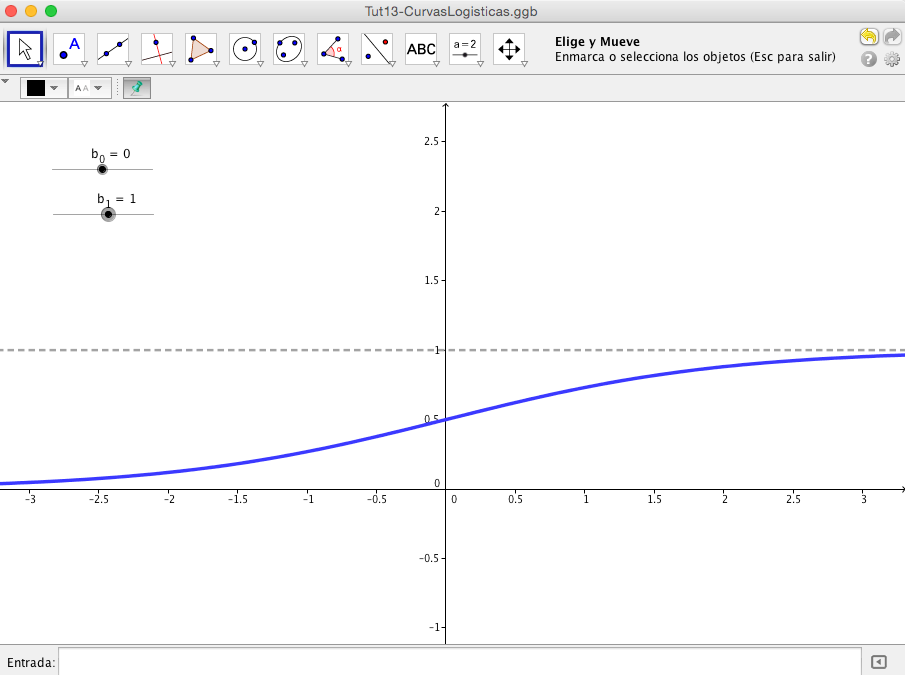
\includegraphics[width=14cm]{../fig/Tut13-CurvasLogisticasGeoGebra.png}
\end{center}
Usa un rato los deslizadores hasta convencerte de que has comprendido el significado de ambos coeficientes.

\section{Estimando los par<U+00E1>metros.}
\label{tut13:sec:EstimandoParametros}

En esta secci<U+00F3>n vamos a aprender a usar el ordenador para obtener estimaciones de los par<U+00E1>metros $b_0$ y $b_1$, como hemos visto en la Secci<U+00F3>n \ref{curso-cap13:sec:EstimacionParametros} (p<U+00E1>g. \pageref{curso-cap13:sec:EstimacionParametros}) del libro.

\subsection{Valores de $b_0$ y $b_1$  mediante m<U+00ED>nimos cuadrados.}
\textcolor{red}{\bf\sc ADVERTENCIA:} Aunque lo hemos avisado en el libro, insistimos. El m<U+00E9>todo que vamos a mostrar aqu<U+00ED> {\bf NO} es el que se usa en regresi<U+00F3>n log<U+00ED>stica y s<U+00F3>lo lo incluimos para que el lector tenga ocasi<U+00F3>n de darse cuenta de que la regresi<U+00F3>n log<U+00ED>stica usa un m<U+00E9>todo distinto del que hemos visto en la regresi<U+00F3>n lineal simple.

Vamos a ver paso a paso como usar el m<U+00E9>todo de m<U+00ED>nimos cuadrados para obtener una curva de la familia log<U+00ED>stica que aproxime a los datos. Los pasos son los mismos que hemos descrito en la Secci<U+00F3>n \ref{curso-cap13:subsection:ParametrosCurvaSigmoideaMedianteMinimosCuadrados} (p<U+00E1>g. \pageref{curso-cap13:subsection:ParametrosCurvaSigmoideaMedianteMinimosCuadrados}) del libro.

\begin{enumerate}
  \item Aplicar la transformaci<U+00F3>n logit a los valores $\hat p_1,\ldots,\hat p_k$. Llamemos $l_1,\ldots,l_k$ a los valores resultantes. Para hacer esto tenemos qu empezar por asegurarnos de que los valores de las probabilidades est<U+00E1>n comprendidos entre $0$ y $1$, estrictamente. La raz<U+00F3>n para hacer esto es que la transformaci<U+00F3>n logit causar<U+00ED>a problemas con cualquier valor igual a $0$ o igual a $1$ (ver Ejercicio \ref{tut13:ejercicio02}). Lo conseguimos mediante una selecci<U+00F3>n adecuada  de los elementos del vector {\tt probabilidades}:

\begin{knitrout}
\definecolor{shadecolor}{rgb}{0.969, 0.969, 0.969}\color{fgcolor}\begin{kframe}
\begin{alltt}
\hlstd{(probsAcotadas} \hlkwb{=} \hlstd{(probabilidades} \hlopt{<} \hlnum{1}\hlstd{)} \hlopt{&} \hlstd{(probabilidades} \hlopt{>} \hlnum{0}\hlstd{))}
\end{alltt}
\begin{verbatim}
## [-10,-9.5]  (-9.5,-9]  (-9,-8.5]  (-8.5,-8]  (-8,-7.5]  (-7.5,-7] 
##      FALSE      FALSE      FALSE      FALSE      FALSE      FALSE 
##  (-7,-6.5]  (-6.5,-6]  (-6,-5.5]  (-5.5,-5]  (-5,-4.5]  (-4.5,-4] 
##      FALSE      FALSE      FALSE      FALSE      FALSE      FALSE 
##  (-4,-3.5]  (-3.5,-3]  (-3,-2.5]  (-2.5,-2]  (-2,-1.5]  (-1.5,-1] 
##       TRUE      FALSE       TRUE       TRUE       TRUE       TRUE 
##  (-1,-0.5]   (-0.5,0]    (0,0.5]    (0.5,1]    (1,1.5]    (1.5,2] 
##       TRUE       TRUE       TRUE       TRUE       TRUE       TRUE 
##    (2,2.5]    (2.5,3]    (3,3.5]    (3.5,4]    (4,4.5]    (4.5,5] 
##       TRUE       TRUE      FALSE      FALSE      FALSE      FALSE 
##    (5,5.5]    (5.5,6]    (6,6.5]    (6.5,7]    (7,7.5]    (7.5,8] 
##      FALSE      FALSE      FALSE      FALSE      FALSE      FALSE 
##    (8,8.5]    (8.5,9]    (9,9.5]   (9.5,10] 
##      FALSE      FALSE      FALSE      FALSE
\end{verbatim}
\end{kframe}
\end{knitrout}
Como ves, los valores de probabilidades entre 0 y 1, que se concentran en lo que hemos llamado la {\em zona de transici<U+00F3>n}, son los que reciben el valor l<U+00F3>gico {\tt TRUE}. Ahora ya podemos aplicar la transformaci<U+00F3>n {\tt logit}:

\begin{knitrout}
\definecolor{shadecolor}{rgb}{0.969, 0.969, 0.969}\color{fgcolor}\begin{kframe}
\begin{alltt}
\hlstd{probab2Odds} \hlkwb{=} \hlkwd{log}\hlstd{(probabilidades[probsAcotadas]}\hlopt{/}\hlstd{(}\hlnum{1}\hlopt{-}\hlstd{probabilidades[probsAcotadas]))}
\end{alltt}
\end{kframe}
\end{knitrout}

\item Lo que hacemos es obtener un modelo de regresi<U+00F3>n lineal simple, ajustado por m<U+00ED>nimos cuadrados, del vector {\tt probab2Odds} frente a las marcas de clase correspondientes. En el Tutorial10 aprendimos a usar la funci<U+00F3>n {\tt lm} de R para calcular los coeficientes $\widetilde b_0$ y $\widetilde b_1$ de la recta de regresi<U+00F3>n
\[l = \widetilde b_0 +\widetilde b_1\cdot w\]

\begin{knitrout}
\definecolor{shadecolor}{rgb}{0.969, 0.969, 0.969}\color{fgcolor}\begin{kframe}
\begin{alltt}
\hlstd{(Oddslm} \hlkwb{=} \hlkwd{lm}\hlstd{(probab2Odds} \hlopt{~} \hlstd{marcasClase[probsAcotadas]))}
\end{alltt}
\begin{verbatim}
## 
## Call:
## lm(formula = probab2Odds ~ marcasClase[probsAcotadas])
## 
## Coefficients:
##                (Intercept)  marcasClase[probsAcotadas]  
##                      0.177                       0.974
\end{verbatim}
\end{kframe}
\end{knitrout}

para los puntos
\[(w_1,l_1),\ldots,(w_k,l_k).\]
Hemos llamado $\widetilde b_0$ y $\widetilde b_1$ a los coeficientes porque, insistimos, el m<U+00E9>todo que estamos exponiendo {\bf no} es el m<U+00E9>todo que aplicaremos en la regresi<U+00F3>n log<U+00ED>stica. Y queremos usar s<U+00ED>mbolos distintos para los valores obtenidos por casa m<U+00E9>todo.

\item Construimos la curva log<U+00ED>stica correspondiente a esos valores $\widetilde b_0$ y $\widetilde b_1$. Esa curva es, desde luego,
\[
  w = \dfrac{e^{\widetilde{b_0} + \widetilde{b_1} v}}{1 + e^{\widetilde{b_0} + \widetilde{b_1} v}}.
\]
Para obtenerla en R podemos definir una funci<U+00F3>n as<U+00ED>:

\begin{knitrout}
\definecolor{shadecolor}{rgb}{0.969, 0.969, 0.969}\color{fgcolor}\begin{kframe}
\begin{alltt}
\hlstd{curvaLogisticaMinCuad} \hlkwb{=} \hlkwa{function}\hlstd{(}\hlkwc{x}\hlstd{)\{}
  \hlstd{b0} \hlkwb{=} \hlstd{Oddslm}\hlopt{$}\hlstd{coefficients[}\hlnum{1}\hlstd{]}
  \hlstd{b1} \hlkwb{=} \hlstd{Oddslm}\hlopt{$}\hlstd{coefficients[}\hlnum{2}\hlstd{]}
  \hlkwd{return}\hlstd{(}\hlkwd{exp}\hlstd{(b0} \hlopt{+} \hlstd{b1} \hlopt{*} \hlstd{x)}\hlopt{/}\hlstd{(}\hlnum{1} \hlopt{+} \hlkwd{exp}\hlstd{(b0} \hlopt{+} \hlstd{b1} \hlopt{*} \hlstd{x)))}
\hlstd{\}}
\end{alltt}
\end{kframe}
\end{knitrout}

que a<U+00F1>adimos al gr<U+00E1>fico de dispersi<U+00F3>n con este comando (f<U+00ED>jate en las opciones {\tt add=TRUE} para a<U+00F1>adir la curva al gr<U+00E1>fico preexistentey \verb#lty="dotted"# para dibujar una curva discontinua):

\begin{knitrout}
\definecolor{shadecolor}{rgb}{0.969, 0.969, 0.969}\color{fgcolor}\begin{kframe}
\begin{alltt}
\hlkwd{points}\hlstd{(marcasClase, probabilidades,} \hlkwc{col}\hlstd{=}\hlstr{"red"}\hlstd{,} \hlkwc{pch}\hlstd{=}\hlnum{2}\hlstd{,} \hlkwc{lwd}\hlstd{=}\hlnum{2}\hlstd{)}
\hlkwd{curve}\hlstd{(curvaLogisticaMinCuad,} \hlkwc{from} \hlstd{=} \hlopt{-}\hlnum{10}\hlstd{,} \hlkwc{to} \hlstd{=} \hlnum{10}\hlstd{,}
      \hlkwc{col}\hlstd{=}\hlstr{"blue"}\hlstd{,} \hlkwc{lwd}\hlstd{=}\hlstr{"2"}\hlstd{,} \hlkwc{add}\hlstd{=}\hlnum{TRUE}\hlstd{,} \hlkwc{lty}\hlstd{=}\hlstr{"dotted"}\hlstd{)}
\end{alltt}
\end{kframe}

{\centering \includegraphics[width=\maxwidth]{figure/pintarCurvaLogisticaMinCuad-1} 

}



\end{knitrout}

\end{enumerate}

Con esto hemos concluido la construcci<U+00F3>n de este modelo para estimar las probabilidades que, insistimos una vez m<U+00E1>s, {\bf NO} es el que se usa en regresi<U+00F3>n log<U+00ED>stica. En la siguiente secci<U+00F3>n construiremos finalmente el modelo de regresi<U+00F3>n log<U+00ED>stica. Cerramos esta secci<U+00F3>n con un ejercicio para ayudarte a reflexionar sobre las caracter<U+00ED>sticas del m<U+00E9>todo que hemos descrito.

\begin{ejercicio}
\label{tut13:ejercicio04}
<U+00BF>Qu<U+00E9> sucede  si agrupamos los valores de otra manaera? Cambia el n<U+00FA>mero de clases y comprueba qu<U+00E9> sucede con los valores estimados $\widetilde b_0$ y $\widetilde b_1$.
%Soluciones en la p<U+00E1>gina \pageref{tut13:ejercicio04:sol}.
\qed
\end{ejercicio}


\section{Regresi<U+00F3>n log<U+00ED>stica:  $b_0$ y $b_1$  mediante maxima verosimilitud.}
\label{tut13:section:ParametrosCurvaSigmoideaMedianteMaximaVerosimilitud}

En esta secci<U+00F3>n vamos a ver c<U+00F3>mo usar el ordenador para obtener las estimaciones de los coeficientesde la curva log<U+00ED>stica usando el m<U+00E9>todo de m<U+00E1>xima verosimilitud, tal como se describe en la Secci<U+00F3>n \ref{curso-cap13:subsection:ParametrosCurvaSigmoideaMedianteMaximaVerosimilitud} del libro (p<U+00E1>g. \pageref{curso-cap13:subsection:ParametrosCurvaSigmoideaMedianteMaximaVerosimilitud}). Primero aprenderemos c<U+00F3>mo usar la funci<U+00F3>n {\tt glm} de R y luego, en un apartado opcional, veremos un m<U+00E9>todo m<U+00E1>s detallado, que puede resultar interesante para quienes quieran adentrarse un poco m<U+00E1>s en las matem<U+00E1>ticas subyacentes al m<U+00E9>todo.

\subsection{La funci<U+00F3>n {\tt glm} de R.}
\label{tut13:subsec:funcionGlm}

En el Tutorial10 conocimos la funci<U+00F3>n {\tt lm} de R, que nos permit<U+00ED>a obtener r<U+00E1>pida y c<U+00F3>modamente la informaci<U+00F3>n relativa a  un modelo de regresi<U+00F3>n lineal simple. La funci<U+00F3>n {\tt glm} (del ingl<U+00E9>s, {\em generalized linear model}) juega un papel parecido con respecto a los modelos lineales generalizados, de los que la regresi<U+00F3>n log<U+00ED>stica es un ejemplo. Por ejemplo, para obtener los coeficientes del modelo log<U+00ED>stico para los datos del Ejemplo \ref{curso-cap13:ejem:EstimacionModeloLogisticoMedianteClases} del libro (p<U+00E1>g. \pageref{curso-cap13:ejem:EstimacionModeloLogisticoMedianteClases}), con el que hemos venido trabajando en los apartados anteriores, usar<U+00ED>amos la funci<U+00F3>n {\tt glm} de esta manera:

\begin{knitrout}
\definecolor{shadecolor}{rgb}{0.969, 0.969, 0.969}\color{fgcolor}\begin{kframe}
\begin{alltt}
\hlstd{(glmXY} \hlkwb{=} \hlkwd{glm}\hlstd{(Y} \hlopt{~} \hlstd{X,} \hlkwc{family} \hlstd{=} \hlkwd{binomial}\hlstd{(}\hlkwc{link} \hlstd{=} \hlstr{"logit"}\hlstd{),} \hlkwc{data} \hlstd{= datos))}
\end{alltt}
\begin{verbatim}
## 
## Call:  glm(formula = Y ~ X, family = binomial(link = "logit"), data = datos)
## 
## Coefficients:
## (Intercept)            X  
##      0.0953       1.0701  
## 
## Degrees of Freedom: 999 Total (i.e. Null);  998 Residual
## Null Deviance:	    1390 
## Residual Deviance: 306 	AIC: 310
\end{verbatim}
\end{kframe}
\end{knitrout}

Como en los modelos lineales, hemos guardado el resultado de {\tt glm} en una variable para facilitar el acceso posterior al modelo. Antes de seguir adelante aplicamos {\tt summary} a ese modelo:
\begin{knitrout}
\definecolor{shadecolor}{rgb}{0.969, 0.969, 0.969}\color{fgcolor}\begin{kframe}
\begin{alltt}
\hlstd{(summGlmXY} \hlkwb{=} \hlkwd{summary}\hlstd{(glmXY))}
\end{alltt}
\begin{verbatim}
## 
## Call:
## glm(formula = Y ~ X, family = binomial(link = "logit"), data = datos)
## 
## Deviance Residuals: 
##     Min       1Q   Median       3Q      Max  
## -2.4259  -0.0891   0.0073   0.1124   2.7190  
## 
## Coefficients:
##             Estimate Std. Error z value Pr(>|z|)    
## (Intercept)   0.0953     0.1468    0.65     0.52    
## X             1.0701     0.0857   12.49   <2e-16 ***
## ---
## Signif. codes:  0 '***' 0.001 '**' 0.01 '*' 0.05 '.' 0.1 ' ' 1
## 
## (Dispersion parameter for binomial family taken to be 1)
## 
##     Null deviance: 1385.62  on 999  degrees of freedom
## Residual deviance:  306.23  on 998  degrees of freedom
## AIC: 310.2
## 
## Number of Fisher Scoring iterations: 8
\end{verbatim}
\end{kframe}
\end{knitrout}
Vemos que, como tambi<U+00E9>n ocurr<U+00ED>a con {\tt lm}, al aplicar {\tt summary} al modelo se obtiene mucha m<U+00E1>s informaci<U+00F3>n que con la salida original de {\tt glm}.  La columna {\tt Estimate} de la tabla {\tt Coefficients} contiene los valores estimados de los coeficientes de la curva log<U+00ED>stica. Y puesto que, {\em ahora s<U+00ED>}, se han obtenido por el m<U+00E9>todo de m<U+00E1>xima verosimilitud, podemos llamar $\hat b_0$ y $\hat b_1$ a esas estimaciones.  Y los coeficientes estimados son:

\begin{knitrout}
\definecolor{shadecolor}{rgb}{0.969, 0.969, 0.969}\color{fgcolor}\begin{kframe}
\begin{alltt}
\hlstd{(b0glm} \hlkwb{=} \hlstd{summGlmXY}\hlopt{$}\hlstd{coefficients[}\hlnum{1}\hlstd{])}
\end{alltt}
\begin{verbatim}
## [1] 0.095265
\end{verbatim}
\begin{alltt}
\hlstd{(b1glm} \hlkwb{=} \hlstd{summGlmXY}\hlopt{$}\hlstd{coefficients[}\hlnum{2}\hlstd{])}
\end{alltt}
\begin{verbatim}
## [1] 1.0701
\end{verbatim}
\end{kframe}
\end{knitrout}

como hemos dicho en el Ejemplo \ref{curso-cap13:ejem:CurvaLogisticaPorDosMetodos} (p<U+00E1>g. \pageref{curso-cap13:ejem:CurvaLogisticaPorDosMetodos}).

Vamos a a<U+00F1>adir la curva log<U+00ED>stica correspondiente a estos coeficientes al diagrama de dispersi<U+00F3>n. Esa curva aparece en la siguiente figura en trazos (opci<U+00F3>n \verb#lty="dashed"#) rojos. El c<U+00F3>digo es muy parecido al que hemos usado antes para la curva que obtuvimos usando m<U+00ED>nimos cuadrados:

\begin{knitrout}
\definecolor{shadecolor}{rgb}{0.969, 0.969, 0.969}\color{fgcolor}\begin{kframe}
\begin{alltt}
\hlkwd{curve}\hlstd{(curvaLogisticaMinCuad,} \hlkwc{from} \hlstd{=} \hlopt{-}\hlnum{10}\hlstd{,} \hlkwc{to} \hlstd{=} \hlnum{10}\hlstd{,}
      \hlkwc{col}\hlstd{=}\hlstr{"blue"}\hlstd{,} \hlkwc{lwd}\hlstd{=}\hlstr{"2"}\hlstd{,} \hlkwc{add}\hlstd{=}\hlnum{TRUE}\hlstd{,} \hlkwc{lty}\hlstd{=}\hlstr{"dotted"}\hlstd{)}
\hlstd{curvaLogisticaGLM} \hlkwb{=} \hlkwa{function}\hlstd{(}\hlkwc{x}\hlstd{)\{}
  \hlkwd{return}\hlstd{(}\hlkwd{exp}\hlstd{(b0glm} \hlopt{+} \hlstd{b1glm} \hlopt{*} \hlstd{x)}\hlopt{/}\hlstd{(}\hlnum{1} \hlopt{+} \hlkwd{exp}\hlstd{(b0glm} \hlopt{+} \hlstd{b1glm} \hlopt{*} \hlstd{x)))}
\hlstd{\}}
\hlkwd{curve}\hlstd{(curvaLogisticaGLM,} \hlkwc{from} \hlstd{=} \hlopt{-}\hlnum{10}\hlstd{,} \hlkwc{to} \hlstd{=} \hlnum{10}\hlstd{,}
      \hlkwc{col}\hlstd{=}\hlstr{"red"}\hlstd{,} \hlkwc{lwd}\hlstd{=}\hlstr{"2"}\hlstd{,} \hlkwc{add}\hlstd{=}\hlnum{TRUE}\hlstd{,} \hlkwc{lty}\hlstd{=}\hlstr{"dashed"}\hlstd{)}
\hlkwd{legend}\hlstd{(}\hlkwc{x}\hlstd{=}\hlstr{"right"}\hlstd{,} \hlkwc{legend}\hlstd{=}\hlkwd{c}\hlstd{(}\hlstr{"M<U+00E1>xima verosimilitud"}\hlstd{,} \hlstr{"M<U+00ED>nimos cuadrados"}\hlstd{),}
       \hlkwc{col} \hlstd{=} \hlkwd{c}\hlstd{(}\hlstr{"red"}\hlstd{,} \hlstr{"blue"}\hlstd{),} \hlkwc{bty}\hlstd{=}\hlnum{1}\hlstd{,} \hlkwc{lty}\hlstd{=}\hlkwd{c}\hlstd{(}\hlstr{"dashed"}\hlstd{,}\hlstr{"dotted"}\hlstd{),}\hlkwc{lwd}\hlstd{=}\hlnum{3}\hlstd{,}\hlkwc{cex}\hlstd{=}\hlnum{1.5}\hlstd{)}
\end{alltt}
\end{kframe}

{\centering \includegraphics[width=\maxwidth]{figure/pintarCurvaLogisticasDosModelos-1} 

}



\end{knitrout}




La figura que hemos obtenido es, esencialmente, la Figura \ref{curso-cap13:fig:CurvaLogisticaPorDosMetodos} del libro (p<U+00E1>g. \pageref{curso-cap13:fig:CurvaLogisticaPorDosMetodos}).

Volviendo a los resultados de {\tt glm}, el lector habr<U+00E1> observado sin duda la gran cantidad de informaci<U+00F3>n que hemos obtenido. Hay una parte de esa informaci<U+00F3>n que va m<U+00E1>s all<U+00E1> de lo que nosotros vamos a aprender en este curso. Pero en el Cap<U+00ED>tulo \ref{curso-cap:RegresionLogistica} y en las siguientes seccione de este tutorial vamos a tratar de llegar tan lejos como nos sea posible en el an<U+00E1>lisis de esa informaci<U+00F3>n.

Para cerrar este apartado, recuerda que los coeficientes $\hat b_0$ y $\hat b_1$ que hemos obtenido con {\tt glm} son, aproximadamente, los que producen un valor m<U+00E1>ximo de la funci<U+00F3>n verosimilitud (no corresponden exactamente al m<U+00E1>ximo porque se han obtenido por un m<U+00E9>todo num<U+00E9>rico). <U+00BF>Y cu<U+00E1>l es ese valor m<U+00E1>ximo de la verosimilitud? En R es muy f<U+00E1>cil obtenerlo a partir del modelo. De hecho, lo que es inmediato es obtener el logaritmo de la verosimilitud:
\begin{knitrout}
\definecolor{shadecolor}{rgb}{0.969, 0.969, 0.969}\color{fgcolor}\begin{kframe}
\begin{alltt}
\hlstd{(logVerosimilitud} \hlkwb{=} \hlkwd{logLik}\hlstd{(glmXY))}
\end{alltt}
\begin{verbatim}
## 'log Lik.' -153.11 (df=2)
\end{verbatim}
\end{kframe}
\end{knitrout}
El resultado incluye varias {\em decoraciones:} un nombre e informaci<U+00F3>n sobre los grados de libertad del modelo (hablaremos de esto m<U+00E1>s adelante). Para eliminar esa informaci<U+00F3>n extra y acceder simplemente al valor del logaritmo de la verosimilitud hacemos un peque<U+00F1>o cambio:
\begin{knitrout}
\definecolor{shadecolor}{rgb}{0.969, 0.969, 0.969}\color{fgcolor}\begin{kframe}
\begin{alltt}
\hlstd{(logVerosimilitud} \hlkwb{=} \hlkwd{logLik}\hlstd{(glmXY)[}\hlnum{1}\hlstd{])}
\end{alltt}
\begin{verbatim}
## [1] -153.11
\end{verbatim}
\end{kframe}
\end{knitrout}

Y ahora la versosimilitud es simplemente:
\begin{knitrout}
\definecolor{shadecolor}{rgb}{0.969, 0.969, 0.969}\color{fgcolor}\begin{kframe}
\begin{alltt}
\hlstd{(verosimilitud} \hlkwb{=} \hlkwd{exp}\hlstd{(logVerosimilitud))}
\end{alltt}
\begin{verbatim}
## [1] 3.1899e-67
\end{verbatim}
\end{kframe}
\end{knitrout}

Por el momento este resultado no parece de mucha utilidad. Al fin y al cabo, lo que nos trajo aqu<U+00ED> era el deseo de estimar los coeficientes de la curva log<U+00ED>stica, mientras que la verosimilitud parec<U+00ED>a s<U+00F3>lo una herramienta para hacer esa estimaci<U+00F3>n. Pero cuando lleguemos a los apartados sobre inferencia en la regresi<U+00F3>n log<U+00ED>stica veremos que este valor de la verosimilitud juega un papel importante.


\begin{ejercicio}
\label{tut13:ejercicio05}

\begin{enumerate}
\item[]

\item Comprueba los valores de $b_0$ y $b_1$ que aparecen en el Ejemplo \ref{curso-cap13:ejem:coeficientesLogisticaVasculopatia} del libro (p<U+00E1>g. \pageref{curso-cap13:ejem:coeficientesLogisticaVasculopatia}) para el modelo que relaciona itb y vasculopat<U+00ED>a.

\item A<U+00F1>ade la curva log<U+00ED>stica al diagrama  de dispersi<U+00F3>n de esos datos y compara con la Figura \ref{curso-cap13:fig:CurvaLogisticaVasculopatia} del libro (p<U+00E1>g. \pageref{curso-cap13:fig:CurvaLogisticaVasculopatia}).

\item Calcula la verosimilitud de ese modelo log<U+00ED>stico.

\end{enumerate}

%Soluciones en la p<U+00E1>gina \pageref{tut13:ejercicio05:sol}.
\qed
\end{ejercicio}


\subsection{Predicci<U+00F3>n con el modelo log<U+00ED>stico.}
\label{tut13:subsec:PrediccionConModeloLogistico}

Desde que introdujimos la idea de modelo en esta parte del curso hemos insistido en varias ocasiones en que una de las finalidades b<U+00E1>sicas de los modelos son las predicciones. En el caso del modelo de regresi<U+00F3>n log<U+00ED>stica las primeras predicciones que podemos obtener del modelo son los {\em valores ajustados} correspondientes  a los datos de la variable explicativa $X$ que hemos usado para construir el modelo. Es decir, que para cada punto $(x_i, y_i)$ de la muestra obtenemos un valor predicho de la probabilidad:
\[\hat\pi(x)=\dfrac{e^{b_0+b_1\cdot x}}{1+e^{b_0+b_1\cdot x}}.\]
Despu<U+00E9>s de usar {\tt glm}, esos valores ajustados de las probabilidades est<U+00E1>n almacenados en un vector de R que es la componente {\tt fitted.values} del modelo. En el ejemplo con el que estamos trabajando, podemos explorar esas predicciones as<U+00ED>:

\begin{knitrout}
\definecolor{shadecolor}{rgb}{0.969, 0.969, 0.969}\color{fgcolor}\begin{kframe}
\begin{alltt}
\hlkwd{head}\hlstd{(glmXY}\hlopt{$}\hlstd{fitted.values)}
\end{alltt}
\begin{verbatim}
##          1          2          3          4          5          6 
## 0.01792953 0.04952345 0.00139781 0.99990542 0.00018127 0.00559471
\end{verbatim}
\begin{alltt}
\hlkwd{tail}\hlstd{(glmXY}\hlopt{$}\hlstd{fitted.values)}
\end{alltt}
\begin{verbatim}
##         995         996         997         998         999        1000 
## 0.000053528 0.999308273 0.274343833 0.999971163 0.002542159 0.362394478
\end{verbatim}
\end{kframe}
\end{knitrout}

En este ejemplo, con una muestra de $n = 1000$ puntos, al representar gr<U+00E1>ficamente esas predicciones el resultado cubre casi completamente la curva log<U+00ED>stica que produce el modelo. Para facilitar la visualizaci<U+00F3>n hemos pintado la curva log<U+00ED>stica con un trazo gris grueso, y en su interior puedes ver, en negro, las probabilidades que predice el modelo para cada valor de $X$:

\begin{knitrout}
\definecolor{shadecolor}{rgb}{0.969, 0.969, 0.969}\color{fgcolor}\begin{kframe}
\begin{verbatim}
## [1] 0.095265
## [1] 1.0701
\end{verbatim}
\end{kframe}

{\centering \includegraphics[width=\maxwidth]{figure/dibujarCurvaLogistica-1} 

}



\end{knitrout}

En el Tutorial10, al estudiar el modelo de regresi<U+00F3>n lineal, tambi<U+00E9>n vimos que se pod<U+00ED>a usar la funci<U+00F3>n {\tt predict} para obtener predicciones del modelo para valores
de $X$ fuera de la muestra. Por ejemplo, para $x=3$ har<U+00ED>amos:

\begin{knitrout}
\definecolor{shadecolor}{rgb}{0.969, 0.969, 0.969}\color{fgcolor}\begin{kframe}
\begin{alltt}
\hlstd{x0} \hlkwb{=} \hlnum{3}
\hlkwd{predict}\hlstd{(glmXY,} \hlkwc{newdata} \hlstd{=} \hlkwd{data.frame}\hlstd{(}\hlkwc{X}\hlstd{=x0))}
\end{alltt}
\begin{verbatim}
##      1 
## 3.3056
\end{verbatim}
\end{kframe}
\end{knitrout}

Pero el valor es mayor que 1... <U+00BF>no est<U+00E1>bamos prediciendo probabilidades? La respuesta es que, por defecto, lo que devuelve {\tt predict} es el valor del t<U+00E9>rmino $b_0 + b_1 x$ para el modelo. Vamos a comprobarlo:

\begin{knitrout}
\definecolor{shadecolor}{rgb}{0.969, 0.969, 0.969}\color{fgcolor}\begin{kframe}
\begin{alltt}
\hlstd{b0glm} \hlopt{+} \hlstd{b1glm} \hlopt{*} \hlstd{x0}
\end{alltt}
\begin{verbatim}
## [1] 3.3056
\end{verbatim}
\end{kframe}
\end{knitrout}

<U+00BF>Y si lo que queremos es la predicci<U+00F3>n de la probabilidad? En ese caso usamos el argumento opcional \verb#type = "response"# de {\tt predict}

\begin{knitrout}
\definecolor{shadecolor}{rgb}{0.969, 0.969, 0.969}\color{fgcolor}\begin{kframe}
\begin{alltt}
\hlkwd{predict}\hlstd{(glmXY,} \hlkwc{newdata} \hlstd{=} \hlkwd{data.frame}\hlstd{(}\hlkwc{X}\hlstd{=x0),} \hlkwc{type} \hlstd{=} \hlstr{"response"}\hlstd{)}
\end{alltt}
\begin{verbatim}
##       1 
## 0.96462
\end{verbatim}
\end{kframe}
\end{knitrout}

El valor por defecto es \verb#type = "link"#  y ya hemos visto que produce como resultado predicciones en la escala del t<U+00E9>rmino lineal $b_0 + b_1 x$. El valor de la probabilidad que hemos obtenido es, desde luego, el mismo que obtendr<U+00ED>amos sustituyendo el valor de $X$ en la curva log<U+00ED>stica del modelo:

\begin{knitrout}
\definecolor{shadecolor}{rgb}{0.969, 0.969, 0.969}\color{fgcolor}\begin{kframe}
\begin{alltt}
\hlkwd{exp}\hlstd{(b0glm} \hlopt{+} \hlstd{b1glm} \hlopt{*} \hlstd{x0)} \hlopt{/} \hlstd{(}\hlnum{1} \hlopt{+} \hlkwd{exp}\hlstd{(b0glm} \hlopt{+} \hlstd{b1glm} \hlopt{*} \hlstd{x0))}
\end{alltt}
\begin{verbatim}
## [1] 0.96462
\end{verbatim}
\end{kframe}
\end{knitrout}

Y, finalmente, tambi<U+00E9>n podemos obtener ese valor usando la funci<U+00F3>n {\tt plogis}, de la que a<U+00FA>n no hemos hablado:

\begin{knitrout}
\definecolor{shadecolor}{rgb}{0.969, 0.969, 0.969}\color{fgcolor}\begin{kframe}
\begin{alltt}
\hlkwd{plogis}\hlstd{(b0glm} \hlopt{+} \hlstd{b1glm} \hlopt{*} \hlstd{x0)}
\end{alltt}
\begin{verbatim}
## [1] 0.96462
\end{verbatim}
\end{kframe}
\end{knitrout}
No vamos a entrar en muchos m<U+00E1>s detalles sobre {\tt plogis} (el lector interesado puede consultar la ayuda). Nos limitaremos a explicar que el valor de {\tt plogis(u)}, para un n<U+00FA>mero $u$, es
\[\mbox{\tt plogis(u)} = \dfrac{e^u}{1 + e^u}\]


\subsection{C<U+00E1>lculo directo del modelo a partir de la funci<U+00F3>n verosimilitud.}
\label{tut13:subsec:calculoDirectoFuncionVerosimilitud}
\noindent{\bf Opcional: esta secci<U+00F3>n puede omitirse en una primera lectura.}\\

En este apartado, en lugar de recurrir a la funci<U+00F3>n {\tt glm} de R, vamos a construir expl<U+00ED>citamente la funci<U+00F3>n verosimilitud y vamos a buscar su valor m<U+00E1>ximo de otra manera. Recuerda que en la Ecuaci<U+00F3>n \ref{curso-cap13:ecu:FuncionVerosimilitudLogistica} del libro (p<U+00E1>g. \ref{curso-cap13:ecu:FuncionVerosimilitudLogistica}) hemos visto que la funci<U+00F3>n verosimilitud se puede expresar as<U+00ED>:

\[
{\cal L}(x_1,x_2,\ldots,x_n, y_1, y_2, \ldots, y_n;b_0, b_1) =\prod_{i:y_i=1}\hat{\pi}(x_i)  \cdot \prod_{i:y_i=0}(1 - \hat{\pi}(x_i))
\]
\[
=\prod_{i:y_i=1} \dfrac{e^{b_0+b_1\cdot x_i}}{1+e^{b_0+b_1\cdot x_i}}
\cdot \prod_{i:y_i=0}\dfrac{1}{1+e^{b_0+b_1\cdot x_i}}
\]

Vamos a empezar por traducir esta expresi<U+00F3>n a R. Recuerda que aqu<U+00ED> pensamos en $b_0, b_1$ como variables, mientras que $X$ e $Y$ son par<U+00E1>metros.

\begin{knitrout}
\definecolor{shadecolor}{rgb}{0.969, 0.969, 0.969}\color{fgcolor}\begin{kframe}
\begin{alltt}
\hlstd{verosimilitud} \hlkwb{=} \hlkwa{function}\hlstd{(}\hlkwc{b}\hlstd{)\{}
    \hlkwd{prod}\hlstd{(}\hlkwd{exp}\hlstd{(b[}\hlnum{1}\hlstd{]} \hlopt{+} \hlstd{b[}\hlnum{2}\hlstd{]} \hlopt{*} \hlstd{X[Y}\hlopt{==}\hlnum{1}\hlstd{])} \hlopt{/}\hlstd{(}\hlnum{1} \hlopt{+} \hlkwd{exp}\hlstd{(b[}\hlnum{1}\hlstd{]} \hlopt{+} \hlstd{b[}\hlnum{2}\hlstd{]} \hlopt{*} \hlstd{X[Y}\hlopt{==}\hlnum{1}\hlstd{])))} \hlopt{*}
    \hlkwd{prod}\hlstd{(}\hlnum{1} \hlopt{/}\hlstd{(}\hlnum{1} \hlopt{+} \hlkwd{exp}\hlstd{(b[}\hlnum{1}\hlstd{]} \hlopt{+} \hlstd{b[}\hlnum{2}\hlstd{]} \hlopt{*} \hlstd{X[Y}\hlopt{==}\hlnum{0}\hlstd{])))}
\hlstd{\}}
\end{alltt}
\end{kframe}
\end{knitrout}

A continuaci<U+00F3>n vamos a representar gr<U+00E1>ficamente esta funci<U+00F3>n verosimilitud. Puesto que es una funci<U+00F3>n de dos variables, su gr<U+00E1>fica es una superficie en el espacio tridimensional. Ya hemos encontrado alguna de estas gr<U+00E1>ficas en otros tutoriales. Y no nos vamos a extender mucho sobre los comandos de R que vamos a utilizar. Los mostraremos simplemente para que el lector interesado sepa por d<U+00F3>nde empezar a buscar si en el futuro necesita profundizar en esto:

\begin{knitrout}
\definecolor{shadecolor}{rgb}{0.969, 0.969, 0.969}\color{fgcolor}\begin{kframe}
\begin{alltt}
\hlcom{# Creamos una malla o reticula de valores de b0, b1 en los que}
\hlcom{# evaluaremos la funcion verosimilitud mediante la funcion outer}
\hlstd{valores_b0} \hlkwb{=} \hlkwd{seq}\hlstd{(}\hlopt{-}\hlnum{0.5}\hlstd{,} \hlnum{0.5}\hlstd{,} \hlkwc{length.out} \hlstd{=} \hlnum{50}\hlstd{)}\hlcom{#seq(25, 35, length.out = 60)}
\hlstd{valores_b1} \hlkwb{=} \hlkwd{seq}\hlstd{(}\hlnum{0.7}\hlstd{,} \hlnum{1.5}\hlstd{,} \hlkwc{length.out} \hlstd{=} \hlnum{50}\hlstd{)}\hlcom{#seq(-38, -28, length.out = 60)}

\hlcom{# Para la representacion que vamos a hacer necesitamos vectorializar}
\hlcom{# la funcion verosimilitud.}
\hlstd{verosimilitud_vect} \hlkwb{=} \hlkwd{Vectorize}\hlstd{(}\hlkwa{function}\hlstd{(}\hlkwc{b0}\hlstd{,} \hlkwc{b1}\hlstd{)}\hlkwd{verosimilitud}\hlstd{(}\hlkwd{c}\hlstd{(b0, b1)))}

\hlcom{# Usando outer calculamos la verosimilitud para cada}
\hlcom{# combinacion de b0 y b1 en la malla que hemos creado}
\hlstd{zp} \hlkwb{=} \hlkwd{outer}\hlstd{(valores_b0, valores_b1, verosimilitud_vect)}

\hlcom{# Y finalmente persp se encarga de crear el grafico tridimensional}
\hlkwd{persp}\hlstd{(valores_b0, valores_b1, zp,}
      \hlkwc{theta}\hlstd{=}\hlnum{45}\hlstd{,} \hlkwc{phi}\hlstd{=}\hlnum{20}\hlstd{,} \hlcom{# angulos de visualizacion}
      \hlkwc{col}\hlstd{=}\hlstr{"lightblue"}\hlstd{,} \hlkwc{xlab}\hlstd{=}\hlstr{"b0"}\hlstd{,} \hlkwc{ylab}\hlstd{=}\hlstr{"b1"}\hlstd{,} \hlkwc{zlab}\hlstd{=}\hlstr{"Verosimilitud"}\hlstd{)}
\end{alltt}
\end{kframe}

{\centering \includegraphics[width=\maxwidth]{figure/graficaVerosimilitud-1} 

}



\end{knitrout}

La figura que hemos obtenido deja claro que la verosimilitud es m<U+00E1>xima para los valores de $b_0$ y $b_1$ que proporciona el m<U+00E9>todo. En el anterior apartado hemos obtenido esos valores usando {\tt glm}. Pero el problema de encontrar valores m<U+00ED>nimos (o m<U+00E1>ximos) de una funci<U+00F3>n es un problema muy general y que se presenta muy a menudo en una colecci<U+00F3>n muy variada de situaciones. No es de extra<U+00F1>ar, por tanto, que exista una parte de las matem<U+00E1>ticas dedicada precisamente a eso. La {\sf Optimizaci<U+00F3>n} estudia los m<U+00E9>todos para localizar esos valores extremos (m<U+00E1>ximos o m<U+00ED>nimos) de una funci<U+00F3>n bajo una serie de condiciones. En R disponemos de varias herramientas de optimizaci<U+00F3>n que en muchas ocasiones son suficientes. Una de esas herramientas es la funci<U+00F3>n {\tt optim}. No podemos extendernos demasiado sobre esta herramienta, porque las posibilidades de configurarla son muy amplias. Nosotros vamos a usar uno de los m<U+00E9>todos de optimizaci<U+00F3>n disponibles, concretamente el m<U+00E9>todo llamado {\sf BFGS} por sus autores, (Broyden, Fletcher, Goldfarb, Shanno). El lector interesado puede encontrar m<U+00E1>s informaci<U+00F3>n en la ayuda de la funci<U+00F3>n {\tt optim} o en el libro (m<U+00E1>s informaci<U+00F3>n usando el enlace)
\begin{center}
\link{https://www.crcpress.com/product/isbn/9781439884485}{{\em Using R for Numerical Analysis in Science and Engineering} de V. Bloomfield}
\end{center}

Para usar ese m<U+00E9>todo debemos proporcionarle a la funci<U+00F3>n {\tt optim} un m<U+00E9>todo para calcular los valores del {\sf gradiente} de la verosimilitud. El gradiente es el vector formado por las dos derivadas parciales:
\[
\operatorname{grad}({\cal L}) = \left(
\dfrac{\partial {\cal L}}{\partial b_0}, \dfrac{\partial {\cal L}}{\partial b_1}
\right)
\]

La funci<U+00F3>n verosimilitud es, como hemos visto, muy complicada. Vamos a simplificar las cosas un poco considerando el logaritmo con signo negativo de la verosimilitud El signo se debe a que {\tt optim}, como la mayor<U+00ED>a de las funciones de optimizaci<U+00F3>n, localiza siempre los valores {\em m<U+00ED>nimos} de la funci<U+00F3>n. Adem<U+00E1>s, en lugar de tratar de encontrar una f<U+00F3>rmula para el gradiente, la librer<U+00ED>a {\tt pracma} de R contiene una funci<U+00F3>n {\tt grad} que permite estimar los valores del gradiente de una funci<U+00F3>n. As<U+00ED> que usaremos esa funci<U+00F3>n para proporcionarle a {\tt optim} los valores del gradiente que requiere el m<U+00E9>todo {\sf BFGS}. Recuerda instalar la llibrer<U+00ED>a {\tt pracma} antes de usarla:

\begin{knitrout}
\definecolor{shadecolor}{rgb}{0.969, 0.969, 0.969}\color{fgcolor}\begin{kframe}
\begin{alltt}
\hlkwd{library}\hlstd{(pracma)}
\end{alltt}


{\ttfamily\noindent\bfseries\color{errorcolor}{\#\# Error in library(pracma): there is no package called 'pracma'}}\begin{alltt}
\hlcom{# Definimos el logaritmo con signo negativo de la funcion verosimilitud}
\hlstd{logVerosmltd} \hlkwb{=} \hlkwa{function}\hlstd{(}\hlkwc{b}\hlstd{)\{}
  \hlopt{-} \hlkwd{log}\hlstd{(}\hlkwd{verosimilitud}\hlstd{(b))}
\hlstd{\}}

\hlcom{# Y usamos grad para estimar su gradiente en un punto b = (b0, b1)}
\hlstd{grad_logVerosmltd} \hlkwb{=} \hlkwa{function}\hlstd{(}\hlkwc{b}\hlstd{)\{}\hlkwd{grad}\hlstd{(logVerosmltd,} \hlkwc{x0} \hlstd{= b)\}}
\end{alltt}
\end{kframe}
\end{knitrout}

Ahora ya estamos listos para usar la funci<U+00F3>n {\tt optim}. Para hacerlo debemos darle un valor inicial aproximado de $b_0$ y $b_1$. Como, en principio, no tenemos ninguna estimaci<U+00F3>n, simplemente tomaremos ambos iguales a $1$. Al tratarse de un m<U+00E9>todo aproximado, otros valores iniciales producir<U+00ED>an resultados ligeramente distintos. Puedes experimentar con otros valores. El resultado de {\tt optim} contiene bastante informaci<U+00F3>n sobre el proceso de optimizaci<U+00F3>n asociado al m<U+00E9>todo {\sf BFGS}:

{\small
\begin{knitrout}
\definecolor{shadecolor}{rgb}{0.969, 0.969, 0.969}\color{fgcolor}\begin{kframe}
\begin{alltt}
\hlstd{(optimizacion} \hlkwb{=}
   \hlkwd{optim}\hlstd{(}\hlkwc{par} \hlstd{=} \hlkwd{c}\hlstd{(}\hlnum{1}\hlstd{,} \hlnum{1}\hlstd{),} \hlkwc{fn} \hlstd{= logVerosmltd,} \hlkwc{gr} \hlstd{= grad_logVerosmltd,} \hlkwc{method}\hlstd{=}\hlstr{"BFGS"}\hlstd{))}
\end{alltt}


{\ttfamily\noindent\bfseries\color{errorcolor}{\#\# Error in gr(par, ...): no se pudo encontrar la funci'on "{}grad"{}}}\end{kframe}
\end{knitrout}
}

La componente {\tt par} del resultado contiene la estimaci<U+00F3>n de los valores $b_0$ y $b_1$ que producen el resultado <U+00F3>ptimo:
\begin{knitrout}
\definecolor{shadecolor}{rgb}{0.969, 0.969, 0.969}\color{fgcolor}\begin{kframe}
\begin{alltt}
\hlstd{optimizacion}\hlopt{$}\hlstd{par}
\end{alltt}


{\ttfamily\noindent\bfseries\color{errorcolor}{\#\# Error in eval(expr, envir, enclos): objeto 'optimizacion' no encontrado}}\end{kframe}
\end{knitrout}
y si comparas con lo que obtuvimos en la secci<U+00F3>n previa usando {\tt glm} ver<U+00E1>s que son los mismos valores:
\begin{knitrout}
\definecolor{shadecolor}{rgb}{0.969, 0.969, 0.969}\color{fgcolor}\begin{kframe}
\begin{alltt}
\hlstd{summGlmXY}\hlopt{$}\hlstd{coefficients}
\end{alltt}
\begin{verbatim}
##             Estimate Std. Error  z value   Pr(>|z|)
## (Intercept) 0.095265    0.14684  0.64877 5.1649e-01
## X           1.070099    0.08567 12.49100 8.3591e-36
\end{verbatim}
\end{kframe}
\end{knitrout}














































































































































